\documentclass[12pt,a4paper]{article}

% ==============================================================================
% PACOTES E CONFIGURAÇÕES DE FORMATAÇÃO (PADRÃO SiTEF / FATEC JALES)
% ==============================================================================
\usepackage[utf8]{inputenc}
\usepackage[T1]{fontenc}
\usepackage[brazil,english]{babel}
\usepackage{mathptmx} % Fonte Times New Roman 12pt
\usepackage[top=2.5cm,bottom=2.5cm,left=2.5cm,right=2.5cm]{geometry}
\usepackage{setspace}
\singlespacing % Espaçamento simples conforme modelo de referência
\usepackage{indentfirst}
\setlength{\parindent}{1.0cm} % Recuo de primeira linha de 1,0 cm
\setlength{\parskip}{0pt}     % Sem espaçamento extra entre parágrafos

% Formatação dos títulos de seções (conforme padrão SiTEF - Sem numeração de subseções)
\usepackage{titlesec}
\titleformat{\section}
  {\normalfont\bfseries\uppercase}{\thesection}{1em}{}

\titlespacing*{\section}{0pt}{18pt}{6pt}

% Pacotes para tabelas, quadros, figuras e código
\usepackage{graphicx}
\usepackage{booktabs}
\usepackage{tabularx}
\usepackage{array}
\usepackage{caption}
\usepackage{subcaption}
\usepackage{enumitem}
\usepackage{microtype}
\usepackage{amsmath,amssymb}
\usepackage{float}       % Permite o modificador [H] para fixação exata
\usepackage{placeins}    % Garante que figuras não ultrapassem seções
\usepackage{xurl}        % Permite quebra automática de URLs longas
\usepackage[hidelinks]{hyperref}

% Configuração de legendas e fontes
\captionsetup{
  font={small},
  labelfont={bf},
  justification=centering,
  singlelinecheck=false,
  skip=4pt
}

% Declaração dos tipos 'Quadro' e 'Gráfico'
\DeclareCaptionType{quadro}[Quadro][Lista de Quadros]
\DeclareCaptionType{grafico}[Gráfico][Lista de Gráficos]

% ==============================================================================
% INÍCIO DO DOCUMENTO
% ==============================================================================
\begin{document}
\selectlanguage{brazil}

% ------------------------------------------------------------------------------
% CABEÇALHO: TÍTULOS, AUTORES, AFILIAÇÃO E ÁREA
% ------------------------------------------------------------------------------
\begin{center}
  {\fontsize{12pt}{14pt}\selectfont \textbf{DESENVOLVIMENTO DE UM SISTEMA DE IDENTIFICAÇÃO BOTÂNICA E GESTÃO DE CUIDADOS COM PLANTAS UTILIZANDO INTELIGÊNCIA ARTIFICIAL}\par}
  \vspace{0.3cm}
  {\fontsize{12pt}{14pt}\selectfont DEVELOPMENT OF A BOTANICAL IDENTIFICATION AND PLANT CARE MANAGEMENT SYSTEM USING ARTIFICIAL INTELLIGENCE\par}
  \vspace{0.4cm}
  
  % Autores
  {\fontsize{12pt}{14pt}\selectfont \textbf{Samuel Henrique Carneiro Pereira$^1$, João Antônio Neves$^2$, Karen Valião de Abreu$^3$, Arthur Pires da Costa$^4$}\par}
  \vspace{0.2cm}
  
  % Afiliações
  {\fontsize{10pt}{12pt}\selectfont 
  $^1$Faculdade de Tecnologia Professor José Camargo -- Fatec Jales, samuel.pereira8@aluno.cps.sp.gov.br\par
  $^2$Faculdade de Tecnologia Professor José Camargo -- Fatec Jales, joao.neves2@aluno.cps.gov.br\par
  $^3$Faculdade de Tecnologia Professor José Camargo -- Fatec Jales, karen.abreu@aluno.cps.sp.gov.br\par
  $^4$Faculdade de Tecnologia Professor José Camargo -- Fatec Jales, arthur.costa01@aluno.cps.sp.gov.br\par
  }
\end{center}

\vspace{0.2cm}
\noindent {\fontsize{12pt}{14pt}\selectfont \textbf{Informação e Comunicação}\par}
\noindent {\fontsize{12pt}{14pt}\selectfont \textbf{Subárea: Banco de Dados, Engenharia e Desenvolvimento de Software}\par}
\vspace{0.4cm}

% ------------------------------------------------------------------------------
% RESUMO E PALAVRAS-CHAVE
% ------------------------------------------------------------------------------
\noindent {\fontsize{12pt}{14pt}\selectfont \textbf{RESUMO}\par}
\vspace{0.1cm}
\noindent {\fontsize{12pt}{14pt}\selectfont Este artigo apresenta o desenvolvimento do ScanPlant, um sistema voltado para a identificação de espécies botânicas e o gerenciamento de cuidados diários de cultivo, projetado para atender entusiastas de jardinagem, estudantes e cultivadores domésticos. O objetivo principal do projeto é solucionar a perda recorrente de plantas decorrente da falta de conhecimento técnico sobre ciclos de rega, luminosidade, tipo de solo e manejo fitossanitário, além de alertar preventivamente sobre os riscos de intoxicação causados por espécies venenosas em ambientes residenciais. A solução foi arquitetada integrando uma API RESTful em C\# (.NET 8) com banco de dados relacional PostgreSQL, uma aplicação web responsiva em React com TypeScript e um aplicativo móvel em React Native com Expo. A identificação das plantas é realizada por meio da API Plant.id com visão computacional, aliada a um assistente virtual conversacional baseado no modelo Google Gemini, com filtros de segurança e moderação de conteúdo. Além da modelagem UML e da avaliação com usuários, realizou-se uma demonstração funcional da versão web publicada, abrangendo autenticação, envio de imagem, retorno probabilístico, alertas de segurança, coleção pessoal e orientação conversacional. O ensaio confirmou a integração entre os módulos e evidenciou a necessidade de interpretar a identificação como apoio informativo, e não como laudo botânico definitivo.\par}
\vspace{0.2cm}
\noindent {\fontsize{12pt}{14pt}\selectfont \textbf{Palavras-chave:} identificação de plantas; inteligência artificial; visão computacional; desenvolvimento de software; gestão de cultivo.\par}
\vspace{0.4cm}

% ------------------------------------------------------------------------------
% ABSTRACT AND KEYWORDS
% ------------------------------------------------------------------------------
\selectlanguage{english}
\noindent {\fontsize{12pt}{14pt}\selectfont \textbf{ABSTRACT}\par}
\vspace{0.1cm}
\noindent {\fontsize{12pt}{14pt}\selectfont This article presents the development of ScanPlant, a software system designed for plant species identification and daily care management, aimed at gardening enthusiasts, students, and home growers. The main goal of the project is to address the recurring loss of plant specimens caused by the lack of technical knowledge regarding watering cycles, sunlight requirements, soil type, and plant care, as well as providing preventive warnings about accidental poisoning from toxic plants in household environments. The solution was architected by integrating a C\# (.NET 8) RESTful API with a PostgreSQL relational database, a responsive React Single Page Application with TypeScript, and a cross-platform mobile application in React Native and Expo. Plant identification is performed using the Plant.id computer vision API, combined with a conversational virtual assistant powered by Google Gemini, equipped with content moderation and botanical safety filters. In addition to UML modeling and user evaluation, a functional demonstration of the deployed web version covered authentication, image submission, probabilistic results, safety warnings, personal collection management, and conversational guidance. The trial confirmed the integration among these modules and highlighted that the identification must be interpreted as decision support rather than a definitive botanical report.\par}
\vspace{0.2cm}
\noindent {\fontsize{12pt}{14pt}\selectfont \textbf{Keywords:} plant identification; artificial intelligence; computer vision; software development; plant care management.\par}
\selectlanguage{brazil}
\vspace{0.4cm}

% ==============================================================================
% 1 INTRODUÇÃO
% ==============================================================================
\section{INTRODUÇÃO}

O cultivo de plantas ornamentais, hortaliças e espécies medicinais em residências e apartamentos cresceu significativamente nos últimos anos, impulsionado pela busca por bem-estar, conforto térmico e maior contato com a natureza nos centros urbanos (Hall; Knuth, 2019). No entanto, grande parte dos cultivadores iniciantes encontra dificuldades consideráveis para manter suas plantas saudáveis ao longo do tempo. A falta de conhecimento técnico sobre a quantidade adequada de rega, a exposição solar recomendada para cada espécie, o tipo de substrato e a identificação precoce de pragas frequentemente resulta na perda das plantas, gerando frustração e abandono da prática (Perez et al., 2021).

Paralelamente aos desafios de manejo, surge uma questão importante relacionada à segurança doméstica: a presença de espécies vegetais tóxicas cultivadas em locais de fácil acesso a crianças e animais de estimação. Dados do Sistema Nacional de Informações Tóxico-Farmacológicas (SINITOX, 2022) indicam que acidentes por intoxicação com plantas venenosas ocorrem rotineiramente em residências brasileiras. Espécies bastante populares na decoração de interiores, como a comigo-ninguém-pode (\textit{Dieffenbachia seguine}), a espada-de-são-jorge (\textit{Sansevieria trifasciata}) e a costela-de-adão (\textit{Monstera deliciosa}), contêm compostos como cristais de oxalato de cálcio que podem causar irritações orais severas, edema e problemas gastrointestinais quando mastigadas ou ingeridas (Botha; Penrith, 2008). Na maioria dos casos, os moradores desconhecem o potencial tóxico das plantas que possuem em seus lares.

Com a evolução recente das técnicas de inteligência artificial, especialmente na área de visão computacional com redes neurais convolucionais e modelos de linguagem generativa, tornou-se viável criar soluções computacionais capazes de reconhecer plantas instantaneamente por meio de fotografias tiradas pelo smartphone e fornecer orientações personalizadas em linguagem natural (LeCun; Bengio; Hinton, 2015; Russell; Norvig, 2022). Embora existam aplicativos no mercado internacional voltados para a identificação botânica, a maioria dessas ferramentas adota modelos agressivos de assinatura paga, possui suporte limitado a dúvidas interativas em português ou foca exclusivamente no viés taxonômico florestal, sem atender às rotinas práticas de cultivo e aos alertas de segurança doméstica.

Diante desse contexto, este trabalho tem como objetivo apresentar o desenvolvimento do ScanPlant, um sistema web e móvel voltado para a identificação fotográfica de espécies botânicas, o gerenciamento de rotinas de rega e o suporte interativo ao cultivo por meio de inteligência artificial. O sistema busca se diferenciar no mercado ao oferecer uma plataforma gratuita e integrada, que alia visão computacional precisa, assistente conversacional inteligente com moderação de conteúdo para triagem de toxicidade e um ambiente de troca de experiências entre cultivadores.

% ==============================================================================
% 2 REFERENCIAL TEÓRICO
% ==============================================================================
\section{REFERENCIAL TEÓRICO}

A aplicação de recursos tecnológicos avançados na botânica tem transformado tarefas manuais de catalogação e diagnóstico vegetal em processos automatizados de alta precisão (Wäldchen; Mäder, 2018). As redes neurais convolucionais (CNNs) representam o estado da arte na classificação de imagens biológicas, pois possuem camadas capazes de aprender automaticamente padrões visuais complexos, como contornos foliares, venações, pigmentações e texturas florais (Goodfellow; Bengio; Courville, 2016; Goëau et al., 2018). Plataformas modernas de classificação, a exemplo da API Plant.id (Plant.id, 2024), utilizam redes convolucionais treinadas em grandes bases de dados mundiais, retornando a probabilidade estatística de acerto, o nome científico, os nomes populares e as características taxonômicas da espécie fotografada.

De forma complementar à visão computacional, os Modelos de Linguagem de Grande Porte (LLMs), como o Google Gemini (Google, 2024), viabilizam a criação de assistentes conversacionais interativos que esclarecem dúvidas sobre cuidados agronômicos em linguagem natural (Russell; Norvig, 2022). Por meio do processamento de linguagem natural, o assistente pode receber perguntas sobre sintomas visuais, tipos de adubação e frequência de rega, devolvendo respostas contextualizadas. Para assegurar a integridade das orientações e mitigar alucinações, o sistema necessita de uma camada intermediária de moderação e segurança de conteúdo, capaz de filtrar mensagens fora do escopo botânico e alertar prontamente em situações de ingestão acidental de espécies perigosas.

No âmbito da engenharia de software, a arquitetura baseada em serviços RESTful consolida-se como padrão para a integração desacoplada entre servidores e clientes multiplataforma (Sommerville, 2011). O framework ASP.NET Core 8 em linguagem C\# (Microsoft, 2024a) disponibiliza uma infraestrutura de alto desempenho com injeção de dependências nativa e controle transacional por meio do Entity Framework Core, enquanto o banco de dados PostgreSQL (Postgresql, 2024) garante a persistência segura, escalável e compatível com consultas relacionais e dados geoespaciais. No desenvolvimento das interfaces com os usuários, a biblioteca React (React, 2024) com TypeScript e Tailwind CSS viabiliza a criação de aplicações web de página única (SPA) ágeis e responsivas, e o React Native com Expo permite o reaproveitamento de lógica para dispositivos móveis Android e iOS.

No que tange à segurança da informação, a proteção das aplicações web fundamenta-se nos princípios de autenticação sem estado utilizando tokens JWT assinados via HMAC-SHA256 (Stallings, 2017). A implementação de práticas recomendadas pelo guia OWASP Top 10 (OWASP, 2021), tais como o armazenamento de senhas com funções de derivação criptográfica (PBKDF2/Identity), o controle de taxa de requisições (\textit{rate limiting}) para prevenção de ataques de negação de serviço e o isolamento de chaves secretas de APIs no lado do servidor, assegura a proteção dos dados dos usuários e a resiliência operacional da plataforma.

A investigação das soluções disponíveis no mercado permitiu identificar as características e lacunas dos principais softwares do segmento botânico. Neste estudo foram analisados quatro sistemas de destaque: \textit{PictureThis} (PictureThis, 2024), \textit{PlantNet} (PlantNet, 2024), \textit{Flora Incognita} (Flora Incognita, 2024) e \textit{Planta} (Planta, 2024). A comparação considerou não apenas a capacidade de reconhecimento de espécies, mas também a gratuidade do acesso, o apoio ao manejo cotidiano, os recursos comunitários e os mecanismos de proteção dos dados do usuário.

O \textit{PictureThis} (PictureThis, 2024) destaca-se pela alta acurácia na identificação botânica e diagnóstico de fitopatologias a partir de imagens foliares. Na Figura 1 visualiza-se a interface de reconhecimento do sistema, onde o aplicativo analisa a fotografia e exibe os dados taxonômicos da planta identificada. Apesar de sua qualidade técnica, o aplicativo adota um modelo comercial restritivo com anúncios constantes e bloqueio de funções básicas por meio de planos de assinatura pagos, além de não contar com um assistente conversacional inteligente e flexível em português.

\begin{figure}[H]
\centering
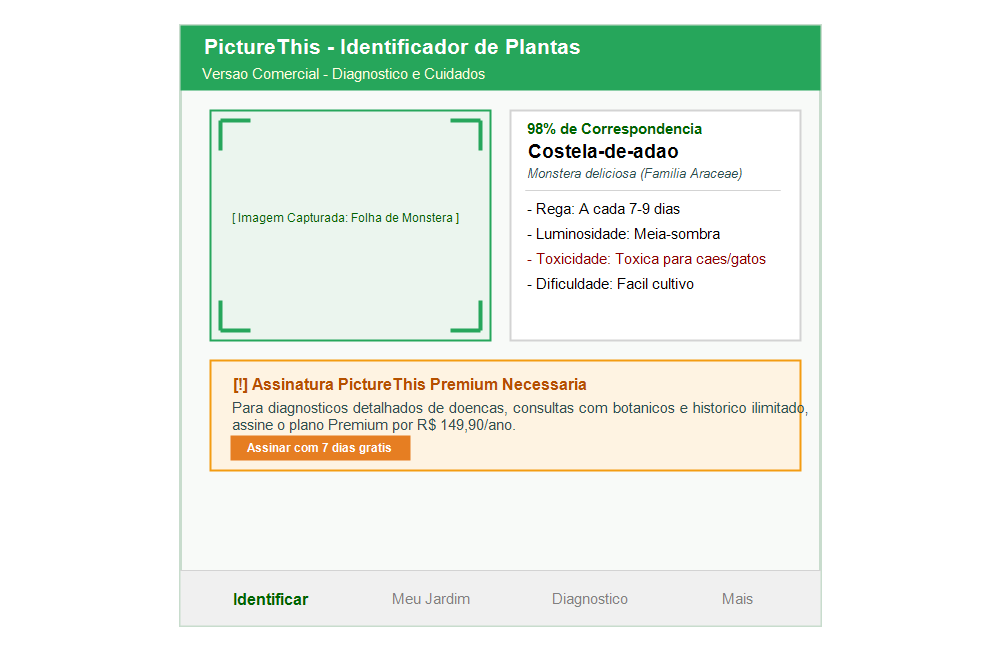
\includegraphics[width=0.75\textwidth]{figuras/figura1_picturethis.png}
\caption{PictureThis: Operação de identificação botânica e diagnóstico de cuidados}
\label{fig:picturethis}
\vspace{2pt}
\small
\noindent Fonte: Elaborada pelos autores com base em PictureThis (2024).
\end{figure}

O \textit{PlantNet} (PlantNet, 2024) constitui um projeto de ciência cidadã amplamente utilizado por botânicos e pesquisadores para inventário da flora selvagem. Na Figura 2 observa-se a tela operacional do aplicativo, que possibilita ao usuário selecionar o órgão vegetal correspondente (folha, flor, fruto, casca) para refinar a busca no banco de dados. Contudo, a plataforma possui foco estritamente acadêmico e taxonômico, não oferecendo ferramentas de controle de rega doméstica, assistente virtual para dúvidas cotidianas nem rede social com controles individuais de privacidade.

\begin{figure}[H]
\centering
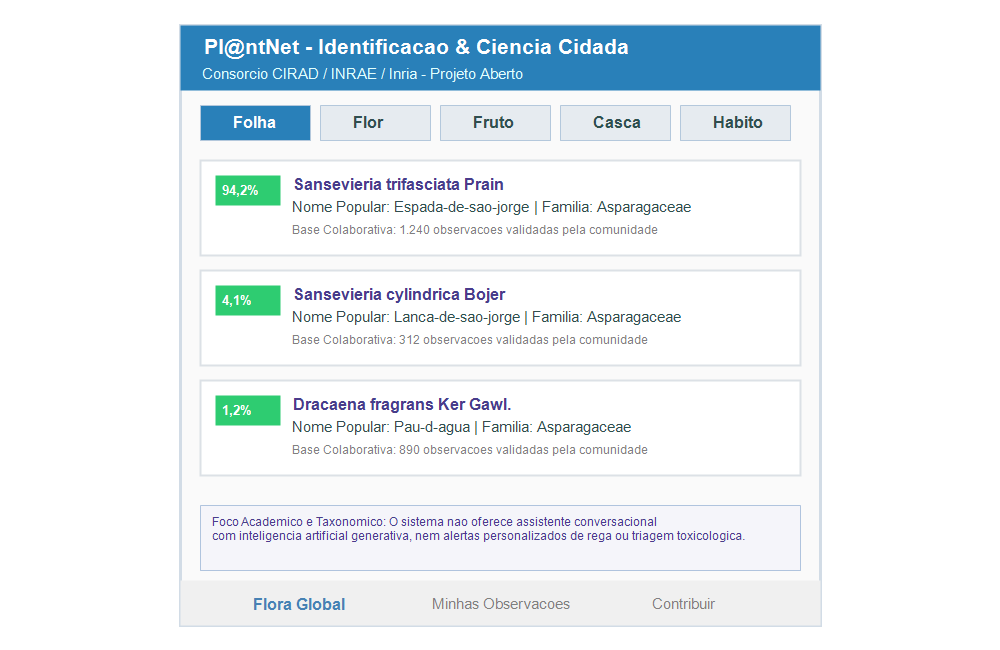
\includegraphics[width=0.75\textwidth]{figuras/figura2_plantnet.png}
\caption{PlantNet: Visão Operacional de identificação taxonômica por órgão vegetal}
\label{fig:plantnet}
\vspace{2pt}
\small
\noindent Fonte: Elaborada pelos autores com base em PlantNet (2024).
\end{figure}

O \textit{Flora Incognita} (Flora Incognita, 2024) apresenta excelente base taxonômica para a flora europeia com fins ecológicos, mas carece de funcionalidades práticas para cultivadores domésticos, como calendários de manutenção e recomendações adaptadas à rotina do usuário. Por outro lado, o aplicativo \textit{Planta} (Planta, 2024) oferece uma estrutura bem elaborada para o agendamento de lembretes e planos de rega, mas restringe a identificação automática por fotos ao plano por assinatura e não possui inteligência conversacional generativa. Essas limitações evidenciam a oportunidade de reunir identificação, acompanhamento e orientação em uma experiência única e acessível.

A análise comparativa entre esses aplicativos e o ScanPlant está consolidada no Quadro 1. Enquanto os sistemas comerciais existentes fragmentam as funcionalidades entre identificação paga, bancos taxonômicos sem suporte a cultivo ou agendas de rega sem inteligência artificial, a proposta do ScanPlant integra o reconhecimento fotográfico por CNNs, o assistente conversacional com IA generativa, a triagem de segurança toxicológica e o catálogo comunitário em uma solução única, acessível e sem custos aos usuários.

\begin{quadro}[H]
\centering
\caption{Comparação das funcionalidades presentes nos sistemas de mercado e no ScanPlant}
\label{quadro:comparacao_sistemas}
\small
\setlength{\tabcolsep}{3pt}
\renewcommand{\arraystretch}{1.12}
\begin{tabularx}{\textwidth}{>{\raggedright\arraybackslash}X *{5}{>{\centering\arraybackslash}p{1.55cm}}}
\toprule
\textbf{Funcionalidade Avaliada} & \textbf{\shortstack{Picture\\This}} & \textbf{PlantNet} & \textbf{\shortstack{Flora\\Incognita}} & \textbf{Planta} & \textbf{\shortstack{Scan\\Plant}} \\
\midrule
Identificação Fotográfica por IA & Sim & Sim & Sim & Sim & Sim \\
Acesso Gratuito sem Assinatura & Não & Sim & Sim & Não & Sim \\
Assistente com IA Generativa & Parcial & Não & Não & Não & Sim \\
Alertas de Toxicidade Doméstica & Limitada & Não & Não & Não & Sim \\
Lembretes de Rega e Cuidados & Sim & Não & Não & Sim & Sim \\
Comunidade e Chat entre Usuários & Não & Não & Não & Não & Sim \\
Controle de Privacidade de Local & Não & Sim & Sim & Não & Sim \\
Proxy Seguro para Chaves de API & Proprie\-tário & Padrão & Padrão & Proprie\-tário & Sim \\
\bottomrule
\end{tabularx}
\vspace{2pt}
\small
\noindent Fonte: Elaborada pelos autores.
\end{quadro}

% ==============================================================================
% 3 METODOLOGIA
% ==============================================================================
\section{METODOLOGIA}

A metodologia adotada neste trabalho classifica-se como aplicada e de desenvolvimento tecnológico, compreendendo o planejamento, a modelagem orientada a objetos e a construção de um software completo para identificação botânica e gestão de cultivo doméstico (Prodanov; Freitas, 2013). O desenvolvimento seguiu as etapas consagradas de engenharia de software sistematizadas por Pressman (2015), iniciando pelo levantamento e especificação dos requisitos, passando pela modelagem arquitetural e estrutural com notação UML, codificação dos serviços de retaguarda e interfaces clientes, até a integração dos módulos de inteligência artificial e mecanismos de segurança da informação.

Para a organização e o acompanhamento das atividades da equipe, adotou-se o framework ágil Scrum (Sutherland; Sutherland, 2019). O cronograma de trabalho foi estruturado em iterações quinzenais (\textit{sprints}), nas quais foram concebidos, implementados e validados os módulos funcionais prioritários: autenticação e controle de perfis de usuário, serviço de identificação por imagem via proxy seguro, assistente botânico generativo com triagem de conteúdo, catálogo pessoal com agendamento de regas, galeria pública da comunidade e troca de mensagens diretas. A gestão visual do fluxo de tarefas foi realizada com quadros Kanban virtuais e repositório Git com controle de versões distribuído.

Os requisitos do sistema foram estabelecidos com base nas demandas práticas observadas no cultivo e na manutenção vegetal em ambientes residenciais e urbanos. No que se refere às funcionalidades essenciais, o software disponibiliza a identificação taxonômica de espécies por meio de fotos capturadas na câmera ou enviadas da galeria, integrando um assistente virtual conversacional especializado em esclarecer dúvidas técnicas sobre irrigação, luminosidade e correção de substrato. Adicionalmente, implementou-se a verificação automatizada de toxicidade com emissão de alertas preventivos, o catálogo personalizado de espécimes com agendamento de regas periódicas, um ambiente colaborativo para publicação de registros botânicos e diálogo entre membros da comunidade, bem como um painel administrativo voltado à auditoria de moderação e ao controle de chaves de acesso a provedores externos de inteligência artificial. Quanto aos atributos de qualidade e arquitetura, priorizou-se o controle de acesso e autenticação sem estado amparado em tokens JWT, o isolamento estrito e a rotação dinâmica de segredos de API na camada servidora para mitigação de vazamentos de credenciais, além de uma taxa reduzida de latência com interface gráfica responsiva e adaptável a múltiplos dispositivos.

Para a representação da análise orientada a objetos e especificação da arquitetura do software, utilizou-se a Linguagem Unificada de Modelagem (UML), empregando o software Astah UML para a elaboração formal dos diagramas estruturais e comportamentais do sistema (Larman, 2007; Booch; Rumbaugh; Jacobson, 2006). Essa modelagem favoreceu a verificação das responsabilidades de cada componente antes da implementação e manteve alinhados os requisitos, as regras de negócio e os fluxos executados pela aplicação.

Na Figura 3 apresenta-se o Diagrama de Classes do ScanPlant desenvolvido no Astah UML. O diagrama detalha as classes do domínio da aplicação, seus atributos tipados, operações essenciais e multiplicidades relacionais. A classe central \texttt{Usuario} gerencia credenciais, preferências, nível de experiência e papel de acesso, relacionando-se com a classe \texttt{Planta} ($1$ para $0..*$) para manutenção das coleções botânicas particulares, com a classe \texttt{Chat} e \texttt{ParticipanteChat} ($1$ para $0..*$) para viabilizar as conversas comunitárias, e com as classes \texttt{EventoModeracao} e \texttt{EventoAuditoriaAdmin} ($1$ para $0..*$) para garantir a conformidade de segurança e rastreabilidade administrativa. A classe \texttt{Planta} encapsula os atributos taxonômicos, coordenadas geográficas, parâmetros de rega e sinalizadores de privacidade (\texttt{naComunidade}, \texttt{localizacaoPublica}). Os laudos diagnósticos de saúde vegetal são modelados pela classe \texttt{DiagnosticoBotanico}, associando a espécie analisada ao índice de confiança estatística e às recomendações agronômicas. Por sua vez, a classe \texttt{CredencialApi} administra a rotação, ativação e registro de falhas das chaves consumidas pelos provedores externos de inteligência artificial.

\begin{figure}[H]
\centering
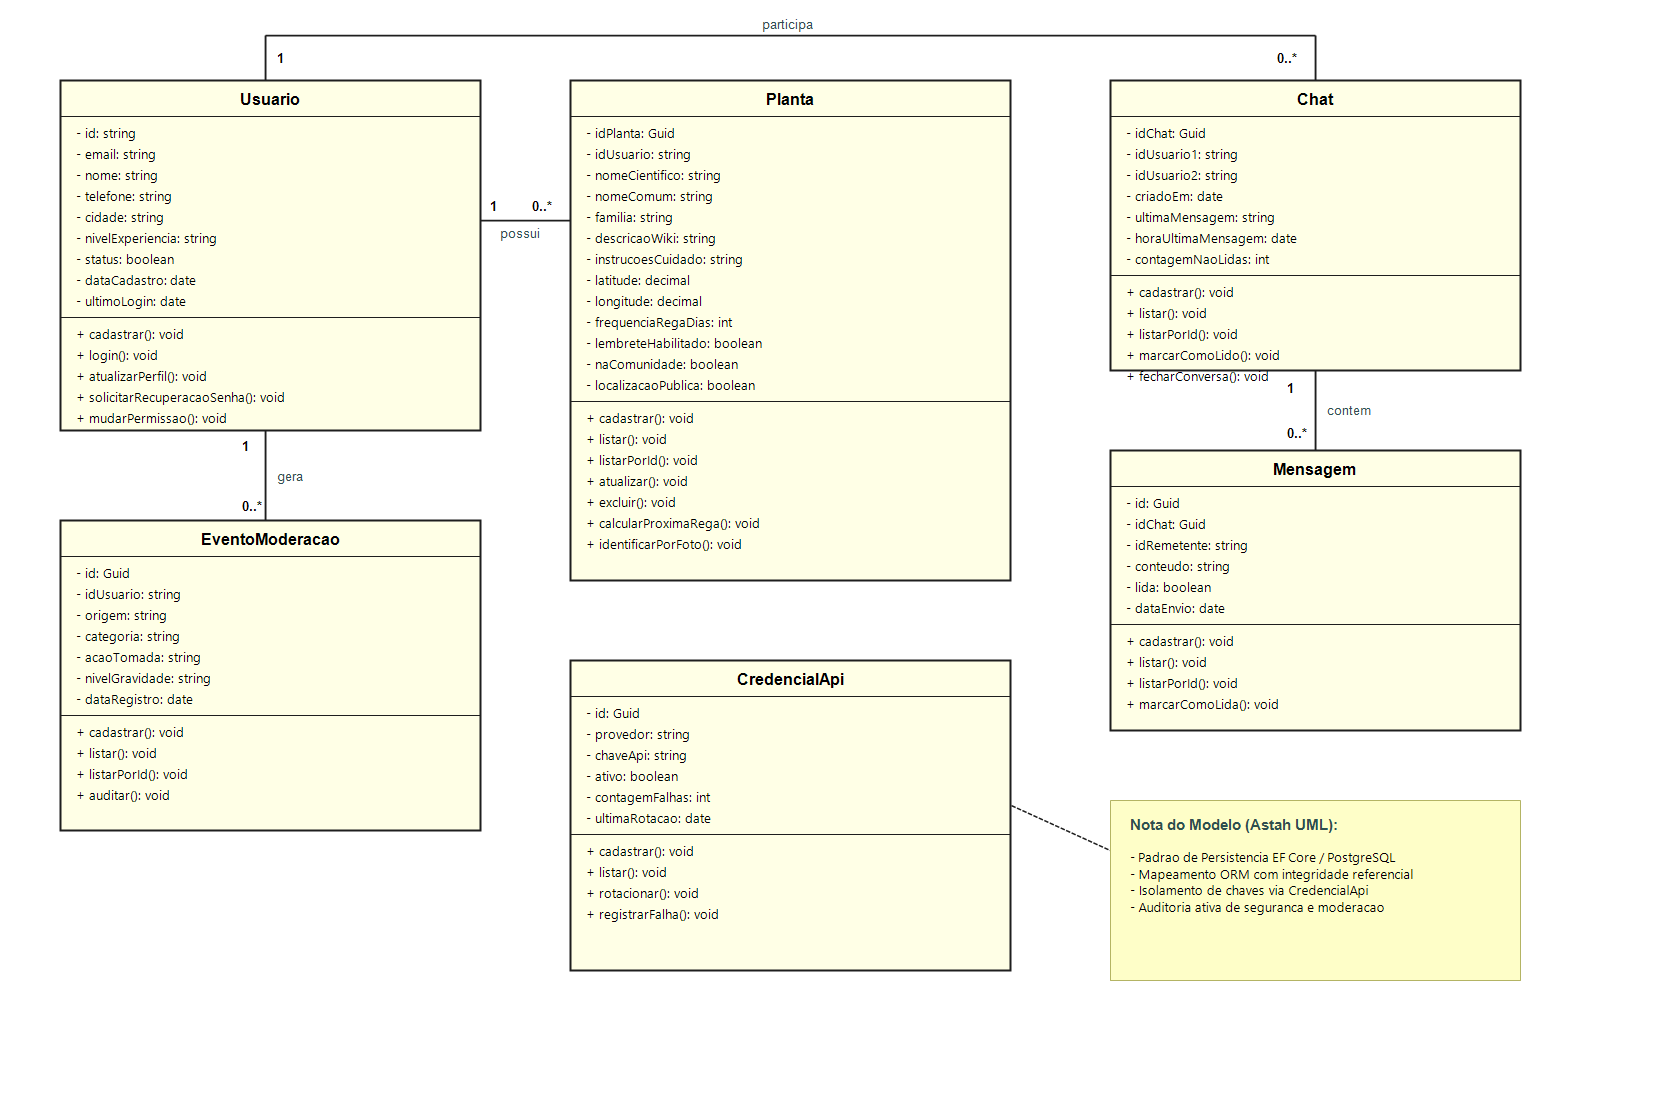
\includegraphics[width=0.94\textwidth]{figuras/figura3_diagrama_classes_astah.png}
\caption{Diagrama de Classes elaborado no software Astah UML}
\label{fig:diagrama_classes}
\vspace{2pt}
\small
\noindent Fonte: Elaborada pelos autores.
\end{figure}

Com base na modelagem de classes, foram definidos os atores do sistema, que representam os papéis exercidos pelos usuários na plataforma. Conforme ilustrado na Figura 4, os atores especializados — Administrador (\texttt{AtorAdm}), Cultivador (\texttt{AtorCultivador}) e Visitante (\texttt{AtorVisitante}) — herdam os atributos e comportamentos da classe base \texttt{AtorUsuario}, garantindo uma estrutura padronizada de controle de acesso e permissões no sistema.

\begin{figure}[H]
\centering
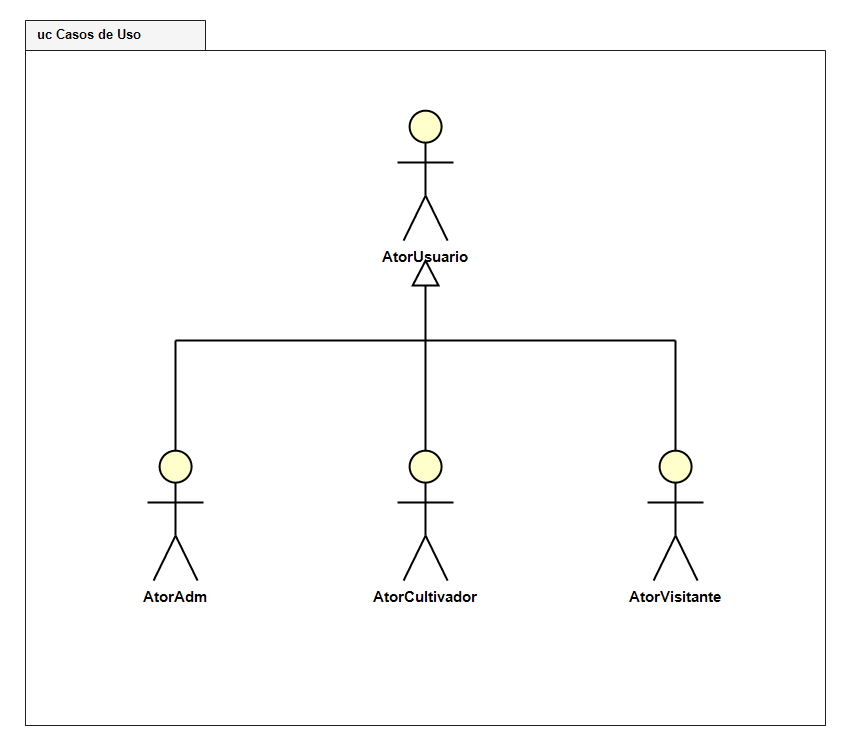
\includegraphics[width=0.55\textwidth]{figuras/figura4_atores_sistema.png}
\caption{Atores do sistema}
\label{fig:atores}
\vspace{2pt}
\small
\noindent Fonte: Elaborada pelos autores.
\end{figure}

No Diagrama de Casos de Uso Geral (Figura 5), ilustram-se as principais interações do cultivador com o sistema ScanPlant, delimitadas pelo limite formal do sistema (\textit{System Boundary}) e orquestradas entre os atores humanos e os serviços computacionais externos. As operações estão organizadas de forma modular em cinco pacotes de funcionalidades: Autenticação e Perfil (cadastro, autenticação, recuperação de credenciais e nível de experiência), Reconhecimento e Diagnóstico (captura fotográfica, identificação de espécies e diagnóstico fitossanitário), Coleção e Cuidados (cadastro de plantas, registro histórico e agendamento de regas), Comunidade e Interação Social (galeria colaborativa e chat direto entre cultivadores) e Administração e Auditoria (gestão de chaves de APIs e visualização de trilhas de moderação). O caso de uso de identificação inclui compulsoriamente a API do Plant.id ($\ll include \gg$), enquanto as consultas ao assistente virtual acionam a API do Google Gemini ($\ll include \gg$). De maneira complementar, a detecção de risco toxicológico estende condicionalmente a emissão de alertas preventivos de emergência ($\ll extend \gg$).

\begin{figure}[H]
\centering
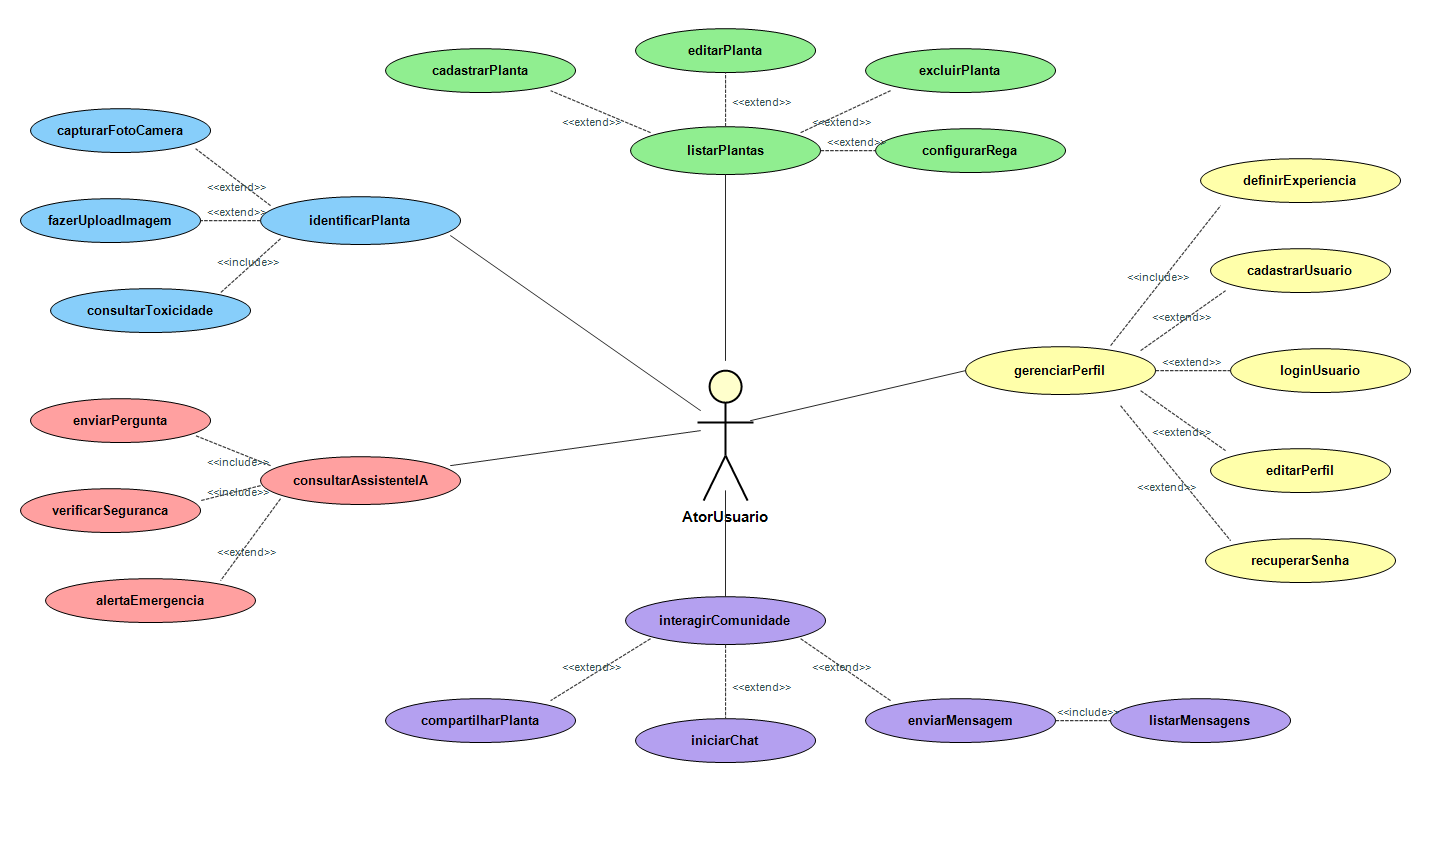
\includegraphics[width=0.92\textwidth]{figuras/figura5_caso_de_uso.png}
\caption{Diagrama de caso de uso geral do sistema ScanPlant}
\label{fig:caso_de_uso}
\vspace{2pt}
\small
\noindent Fonte: Elaborada pelos autores.
\end{figure}

Na Figura 6 apresenta-se o diagrama de sequência do sistema, detalhando o fluxo de processamento e enriquecimento da identificação botânica. A imagem enviada pelo aplicativo cliente é recebida pelo \texttt{PlantIdentificationController}, que valida os parâmetros e aciona o \texttt{ApiCredentialService} para recuperar a credencial ativa do provedor. A requisição é despachada de forma segura para a API do Plant.id, cuja resposta taxonômica é interceptada e enriquecida pelo serviço de segurança com informações de toxicidade e orientações de emergência antes de ser devolvida ao usuário.

\begin{figure}[H]
\centering
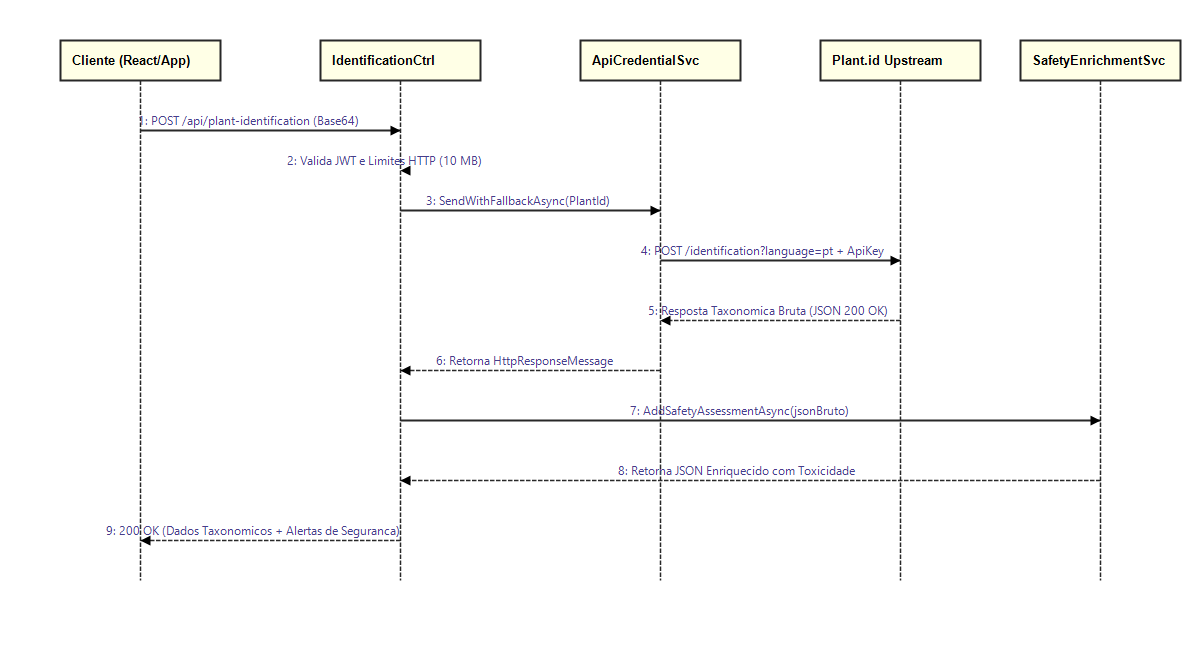
\includegraphics[width=0.82\textwidth]{figuras/figura6_diagrama_sequencia.png}
\caption{Diagrama de sequência do fluxo de identificação e enriquecimento botânico}
\label{fig:sequencia}
\vspace{2pt}
\small
\noindent Fonte: Elaborada pelos autores.
\end{figure}

Para a implementação da solução, a aplicação servidora (back-end) foi desenvolvida em linguagem C\# com o framework ASP.NET Core 8 (Microsoft, 2024a), estruturada segundo as boas práticas da arquitetura RESTful com injeção de dependências nativa e controle de rotas seguras. A persistência de dados e o controle de transações foram estabelecidos com o Entity Framework Core sobre o banco de dados relacional PostgreSQL (Postgresql, 2024), garantindo integridade referencial, consultas otimizadas e resiliência nas conexões. A aplicação cliente (front-end) foi construída em TypeScript utilizando React 18 e Tailwind CSS para navegadores web, e React Native com a plataforma Expo para dispositivos móveis, comunicando-se com o servidor exclusivamente por meio de requisições HTTP serializadas no formato JSON.

A integração dos módulos de inteligência artificial opera por meio de proxies seguros no servidor. A identificação taxonômica consome a API do Plant.id (Plant.id, 2024), enquanto o assistente conversacional utiliza o modelo generativo Google Gemini (Google, 2024). Antes de encaminhar as consultas ao modelo de linguagem, o serviço \texttt{ContentSafetyService} executa a classificação de intenções em categorias específicas (botânica, ingestão acidental perigosa, substâncias controladas ou ofensas), bloqueando termos impróprios e emitindo instruções imediatas de segurança em cenários de suspeita de intoxicação.

Essa arquitetura integrada e modular assegura que o ScanPlant opere com alto desempenho, segurança e confiabilidade, estabelecendo uma base sólida de engenharia de software para o suporte ao cultivo de plantas e à prevenção de acidentes domésticos.

% ==============================================================================
% 4 ANÁLISE E DISCUSSÃO DOS RESULTADOS
% ==============================================================================
\section{ANÁLISE E DISCUSSÃO DOS RESULTADOS}

A avaliação de sistemas computacionais interativos voltados ao público em geral exige a investigação empírica do comportamento dos usuários, de suas necessidades práticas no mundo real e de como a tecnologia concebida responde aos desafios cotidianos (Pressman, 2015). Esta seção apresenta o funcionamento da solução desenvolvida, as regras de negócio implementadas e a análise quantitativa e qualitativa detalhada dos dados coletados na pesquisa de validação empírica realizada com 53 respondentes ($N = 53$), correlacionando os achados às diretrizes da literatura técnica e científica.

\vspace{0.3cm}
\noindent \textbf{Apresentação do Sistema Desenvolvido e Dinâmica Operacional}\par
\vspace{0.1cm}

Para complementar a descrição arquitetural com evidências observáveis de funcionamento, foi conduzido um ensaio controlado na versão web pública do ScanPlant em 4 de setembro de 2026 (ScanPlant, 2026). O procedimento foi executado em navegador para computador e seguiu um roteiro encadeado: criação de uma conta de teste, leitura das orientações iniciais, acesso ao painel, seleção de uma fotografia botânica, submissão ao serviço de identificação, interpretação do resultado, configuração de lembrete, armazenamento na coleção e consulta ao assistente. A adoção de um percurso único permitiu verificar se as informações produzidas em uma etapa permaneciam disponíveis nas etapas seguintes, aspecto essencial em sistemas que integram reconhecimento por imagem, persistência de dados e orientação automatizada.

As Figuras \ref{fig:login} e \ref{fig:cadastro} apresentam, respectivamente, as portas de entrada para usuários já registrados e para novos usuários. A tela de autenticação concentra apenas as credenciais necessárias, oferece recuperação de senha e informa o uso de conexão protegida. O cadastro explicita requisitos mínimos para a senha antes do envio, o que reduz erros de preenchimento e torna a política de acesso compreensível no próprio contexto de uso.

\begin{figure}[H]
\centering
\begin{subfigure}[t]{0.49\textwidth}
  \centering
  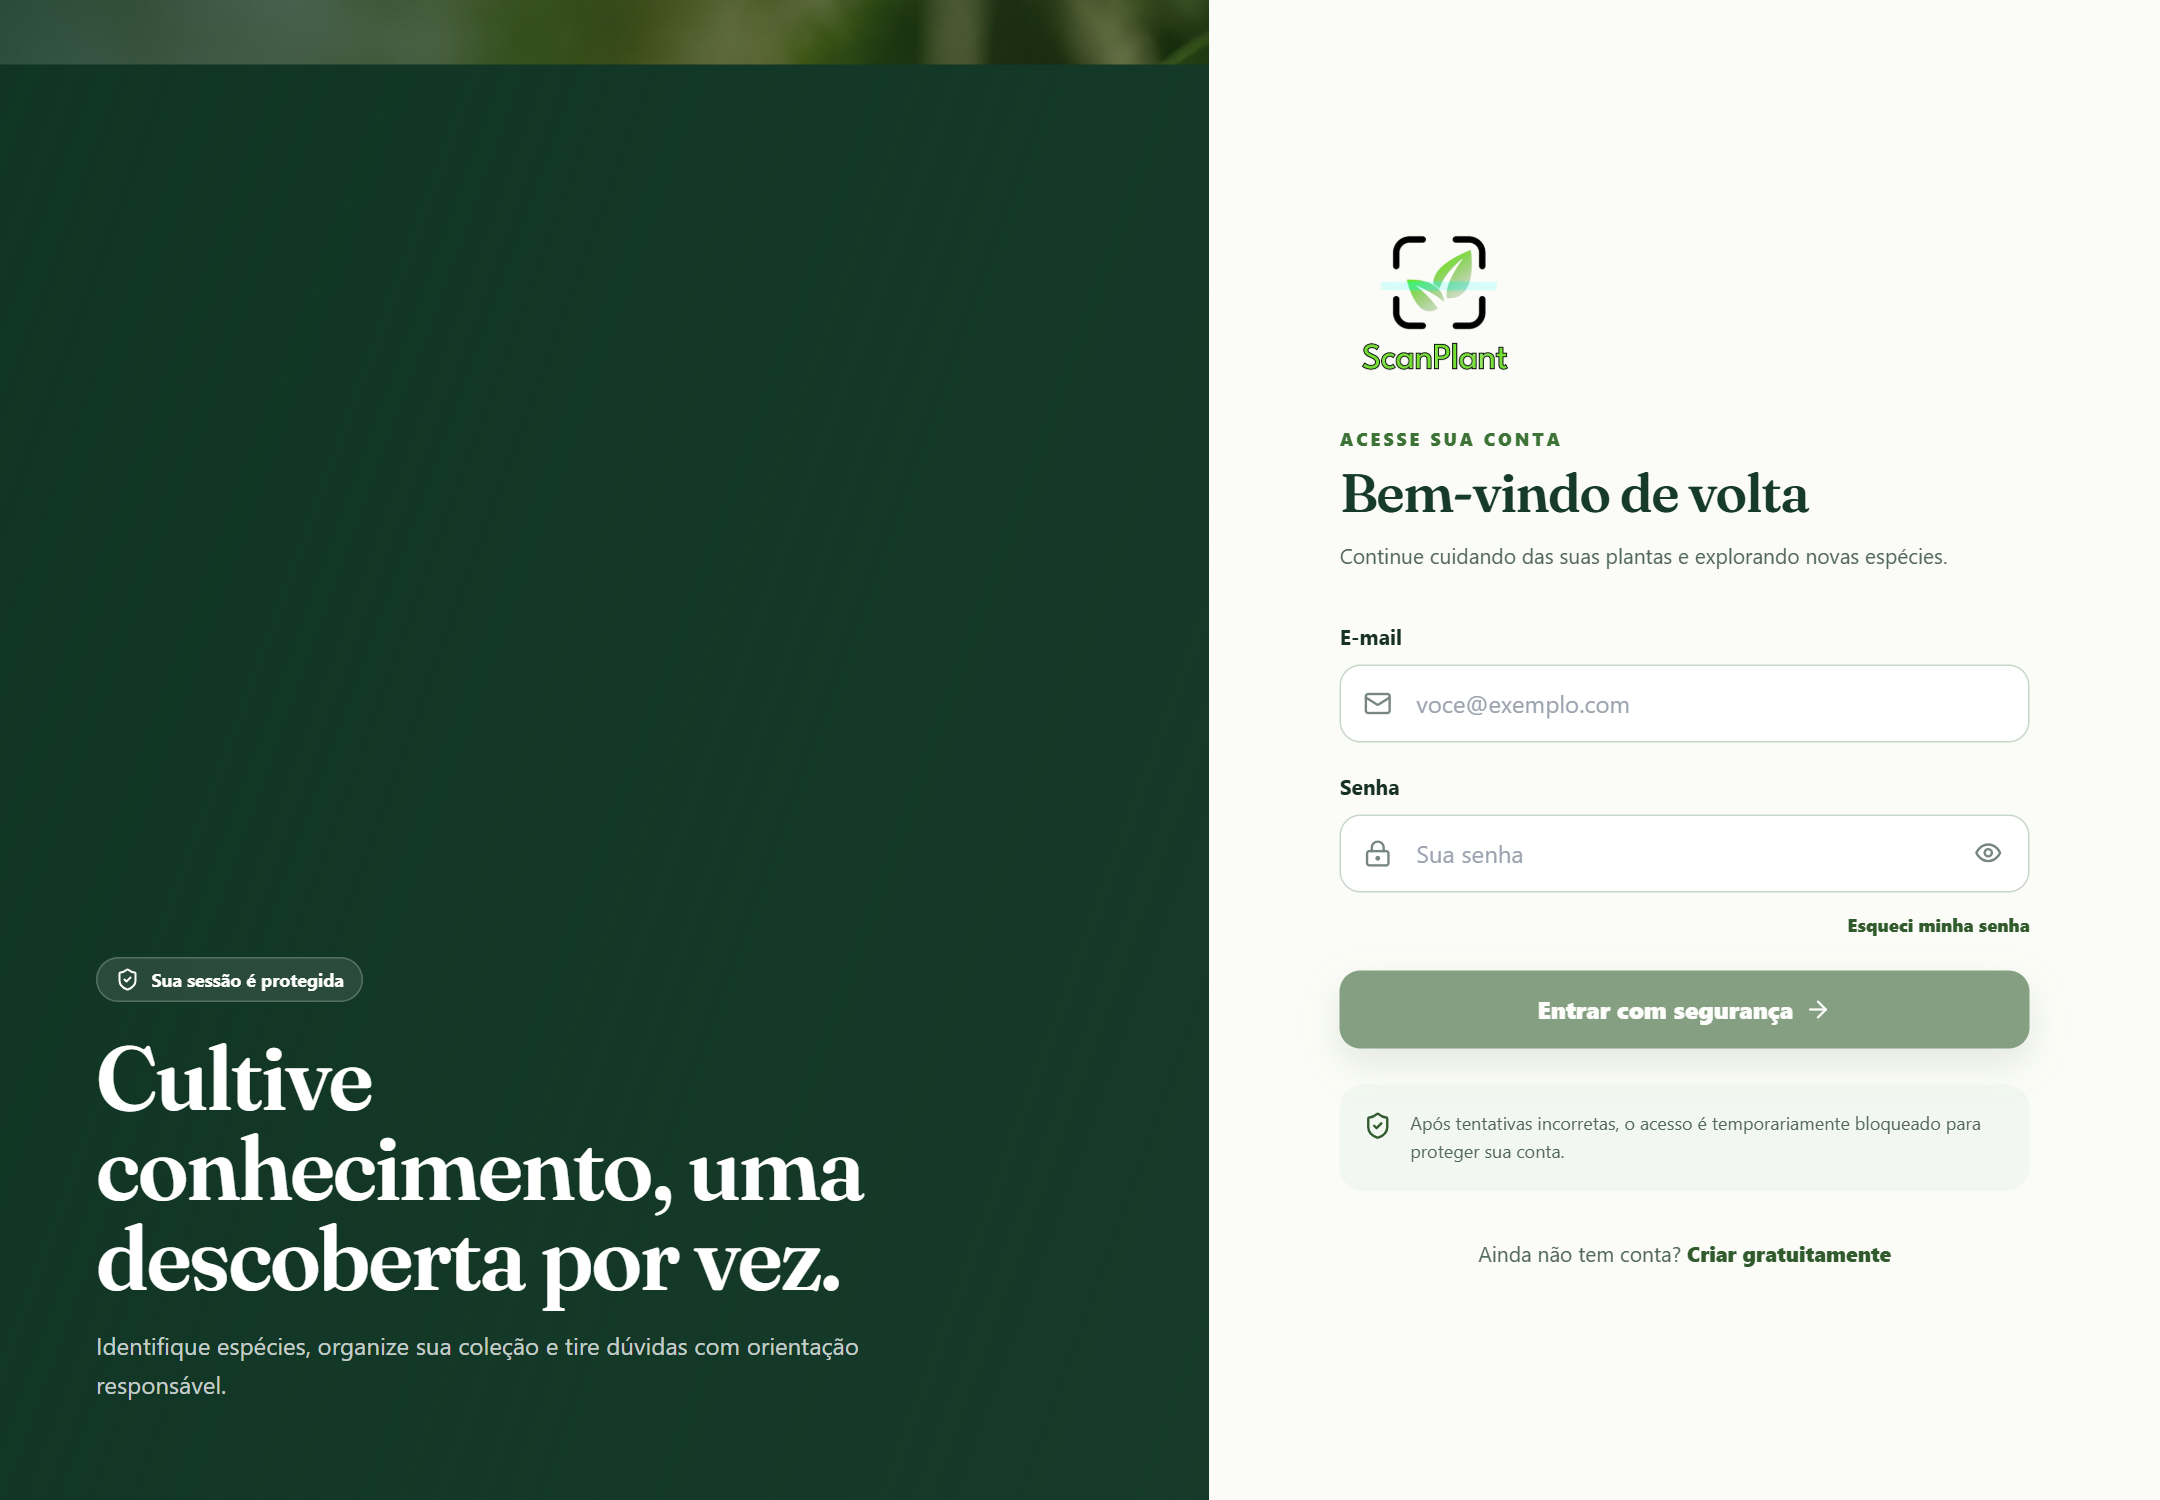
\includegraphics[width=\textwidth]{figuras/sistema/figura7_login.png}
  \caption{Tela de login da versão web publicada}
  \label{fig:login}
\end{subfigure}\hfill
\begin{subfigure}[t]{0.49\textwidth}
  \centering
  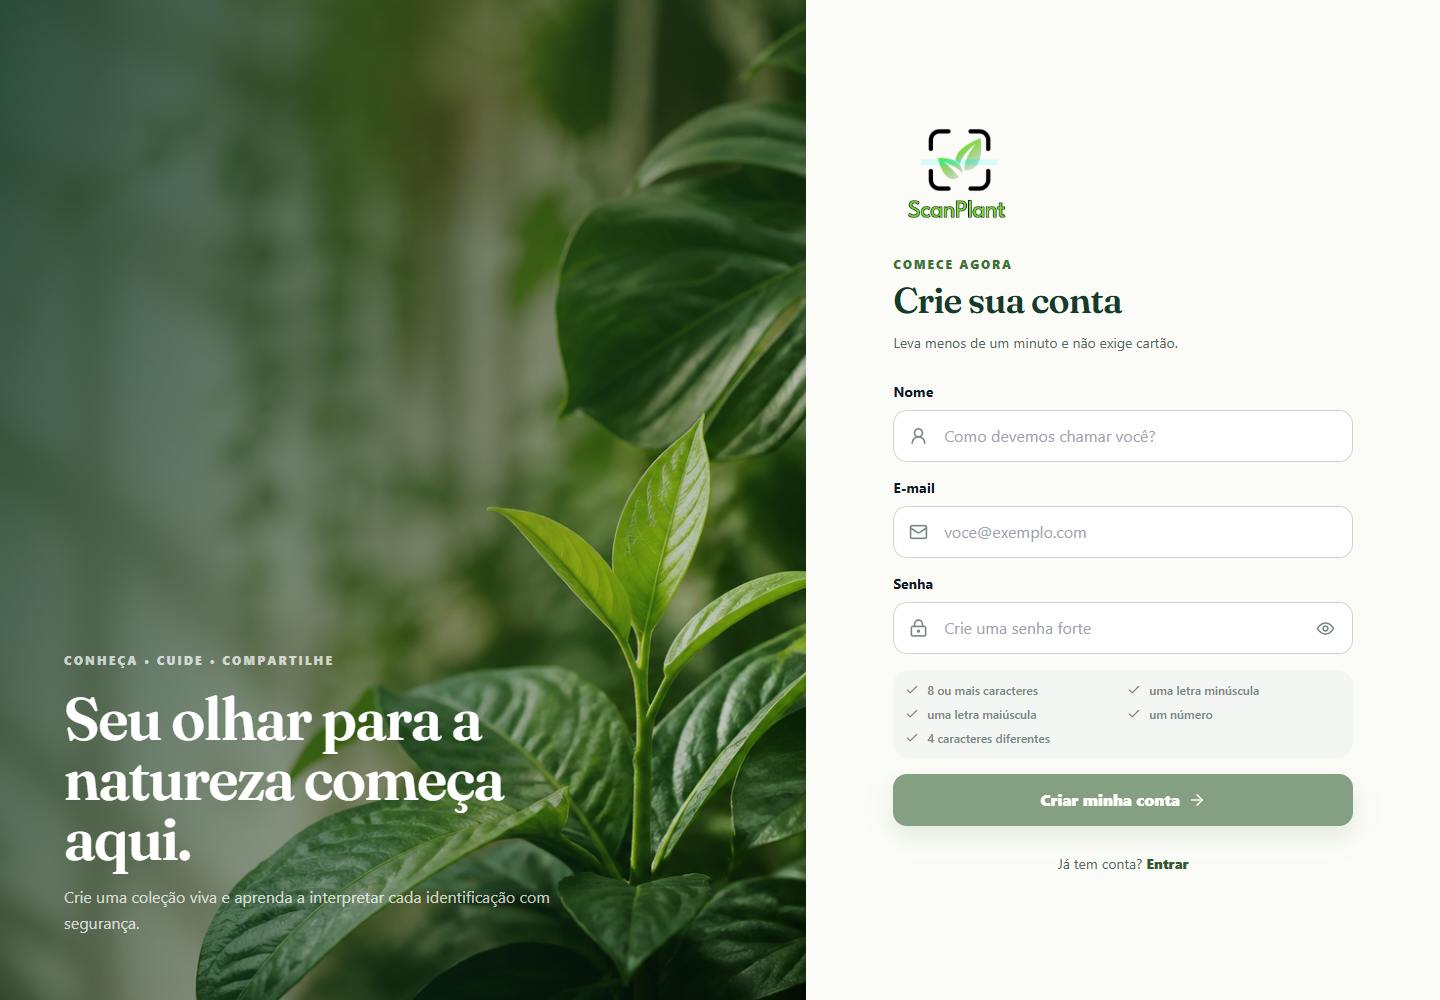
\includegraphics[width=\textwidth]{figuras/sistema/figura8_cadastro.png}
  \caption{Tela de cadastro e requisitos de senha}
  \label{fig:cadastro}
\end{subfigure}
\caption{Fluxo inicial de acesso ao ScanPlant}
\vspace{2pt}
\small
\noindent Fonte: Elaborada pelos autores a partir da versão publicada do ScanPlant (2026).
\end{figure}

Após o primeiro acesso, a aplicação apresenta as orientações reproduzidas na Figura \ref{fig:primeiros_passos}. A sequência ``capture, analise, cuide'' explica o percurso principal e informa que a identificação possui natureza probabilística, além de destacar limites relacionados a consumo, uso medicinal e situações de urgência.

\begin{figure}[H]
\centering
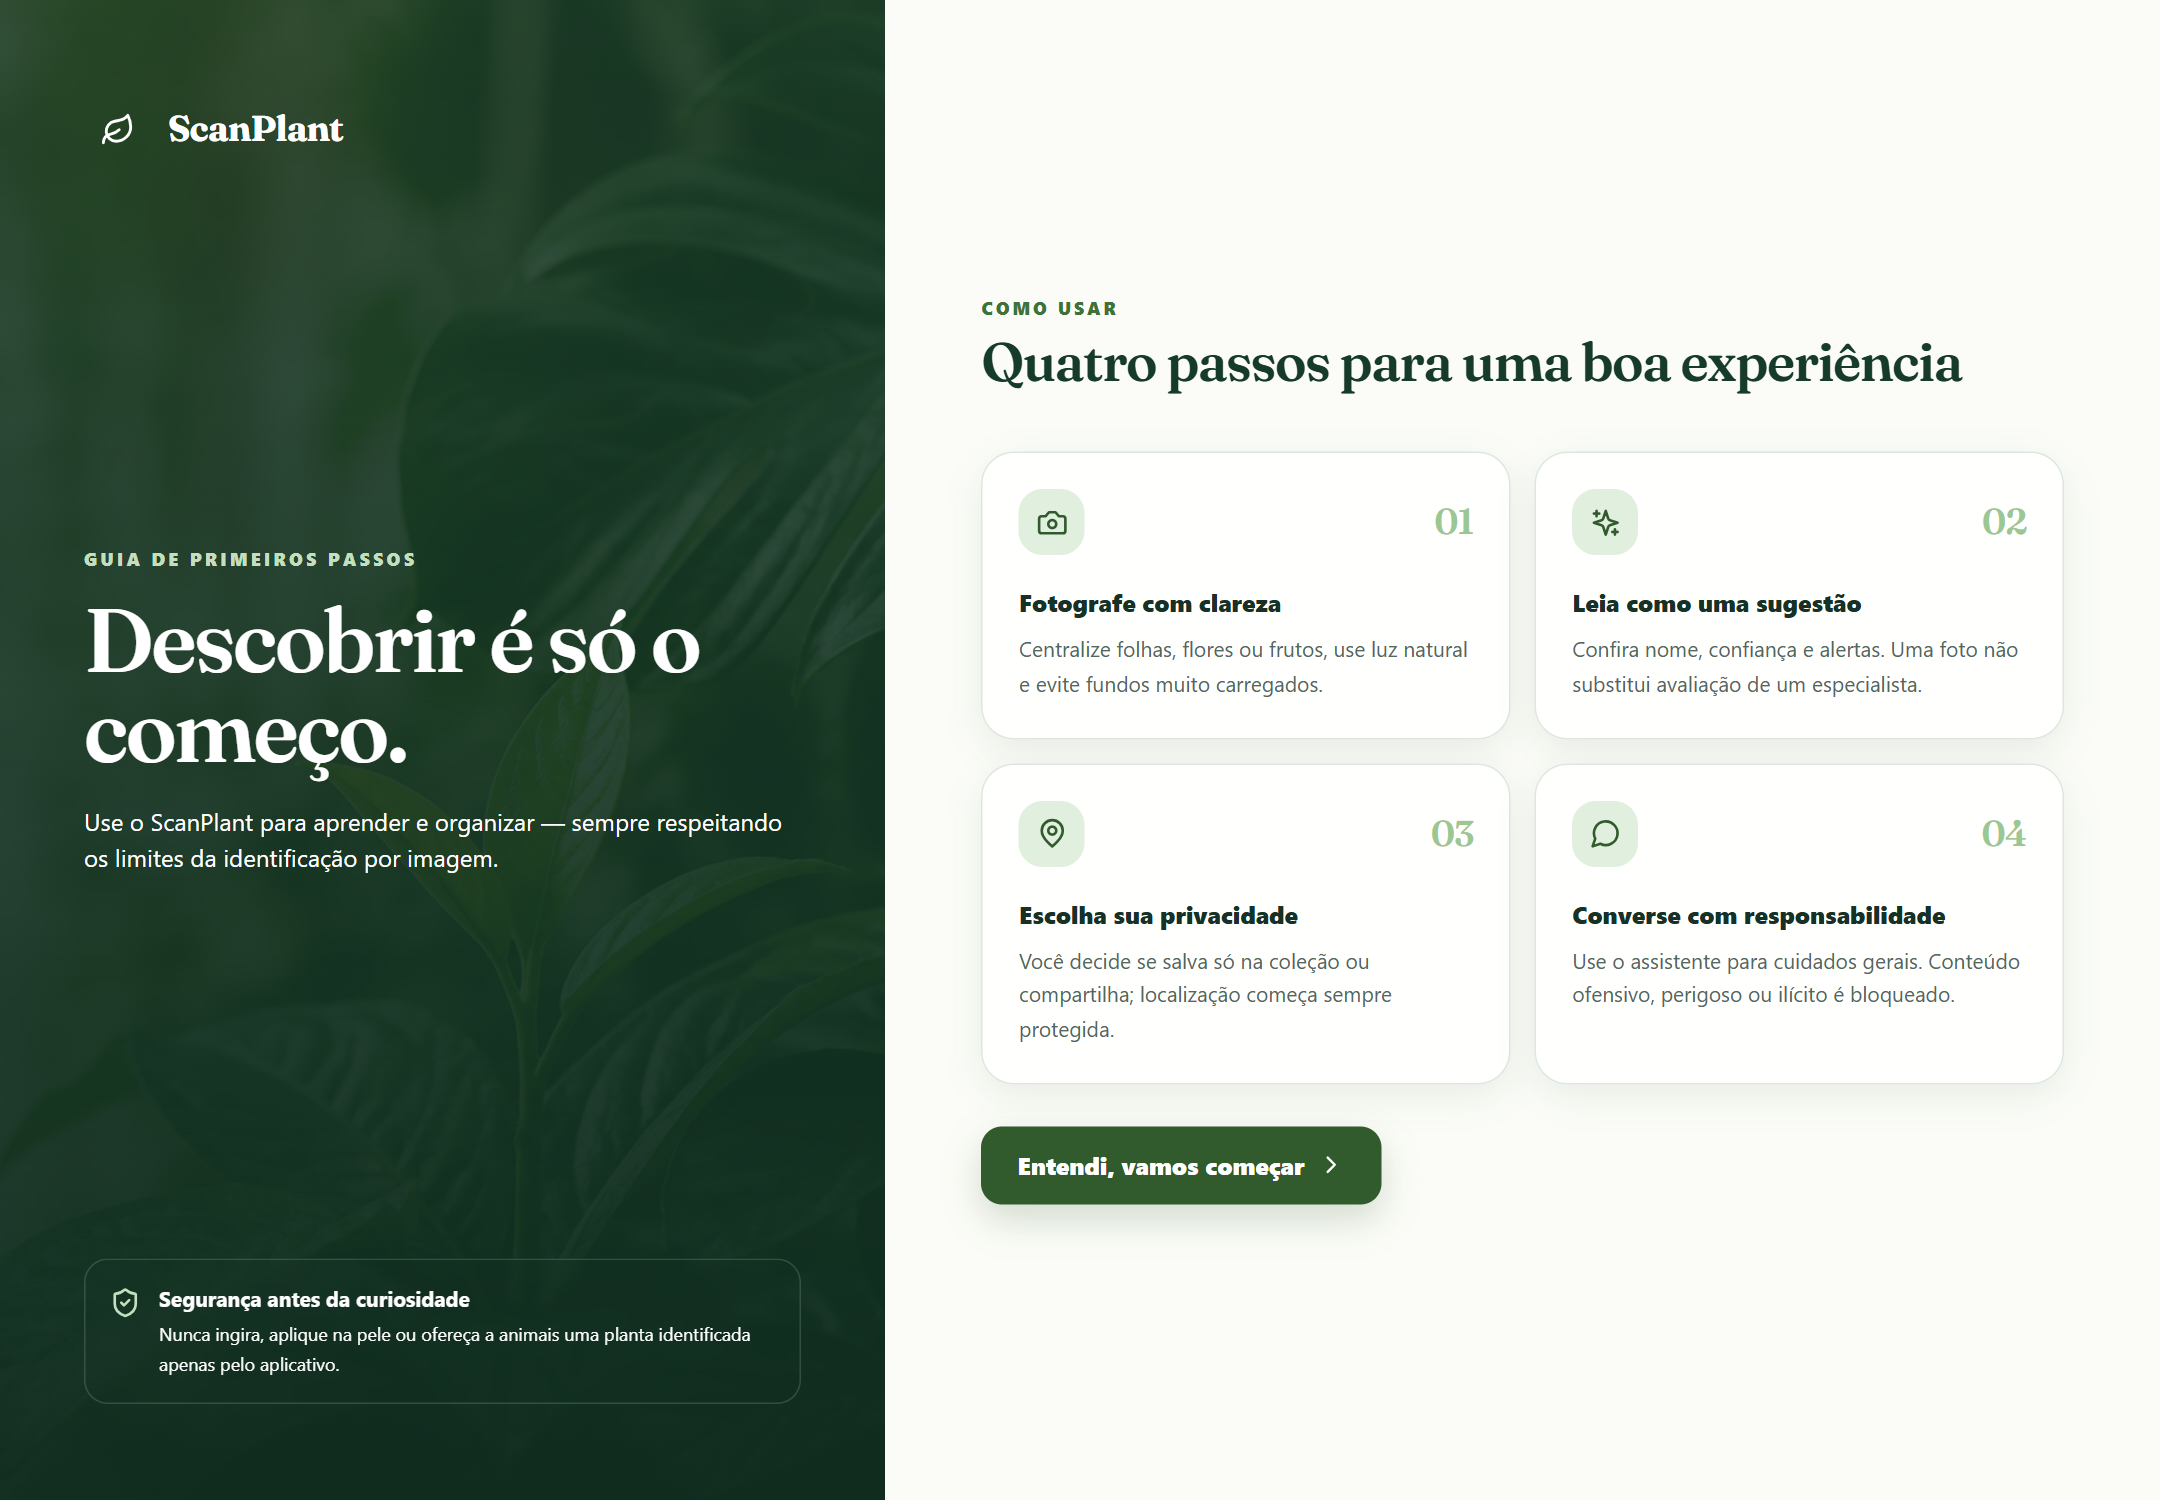
\includegraphics[width=0.80\textwidth]{figuras/sistema/figura9_primeiros_passos.png}
\caption{Orientações de primeiros passos e limites de uso do sistema}
\label{fig:primeiros_passos}
\vspace{2pt}
\small
\noindent Fonte: Elaborada pelos autores a partir da versão publicada do ScanPlant (2026).
\end{figure}

O painel principal, reproduzido na Figura \ref{fig:dashboard}, funciona como ponto de convergência dos módulos. Os atalhos para identificação, exploração, coleção e assistente permanecem disponíveis na navegação lateral, enquanto os cartões centrais destacam tarefas frequentes e o estado da coleção do usuário. A hierarquia visual observada favorece o acesso direto às ações principais e mantém informações de segurança em área visível, sem exigir conhecimento prévio da estrutura interna da aplicação.

\begin{figure}[H]
\centering
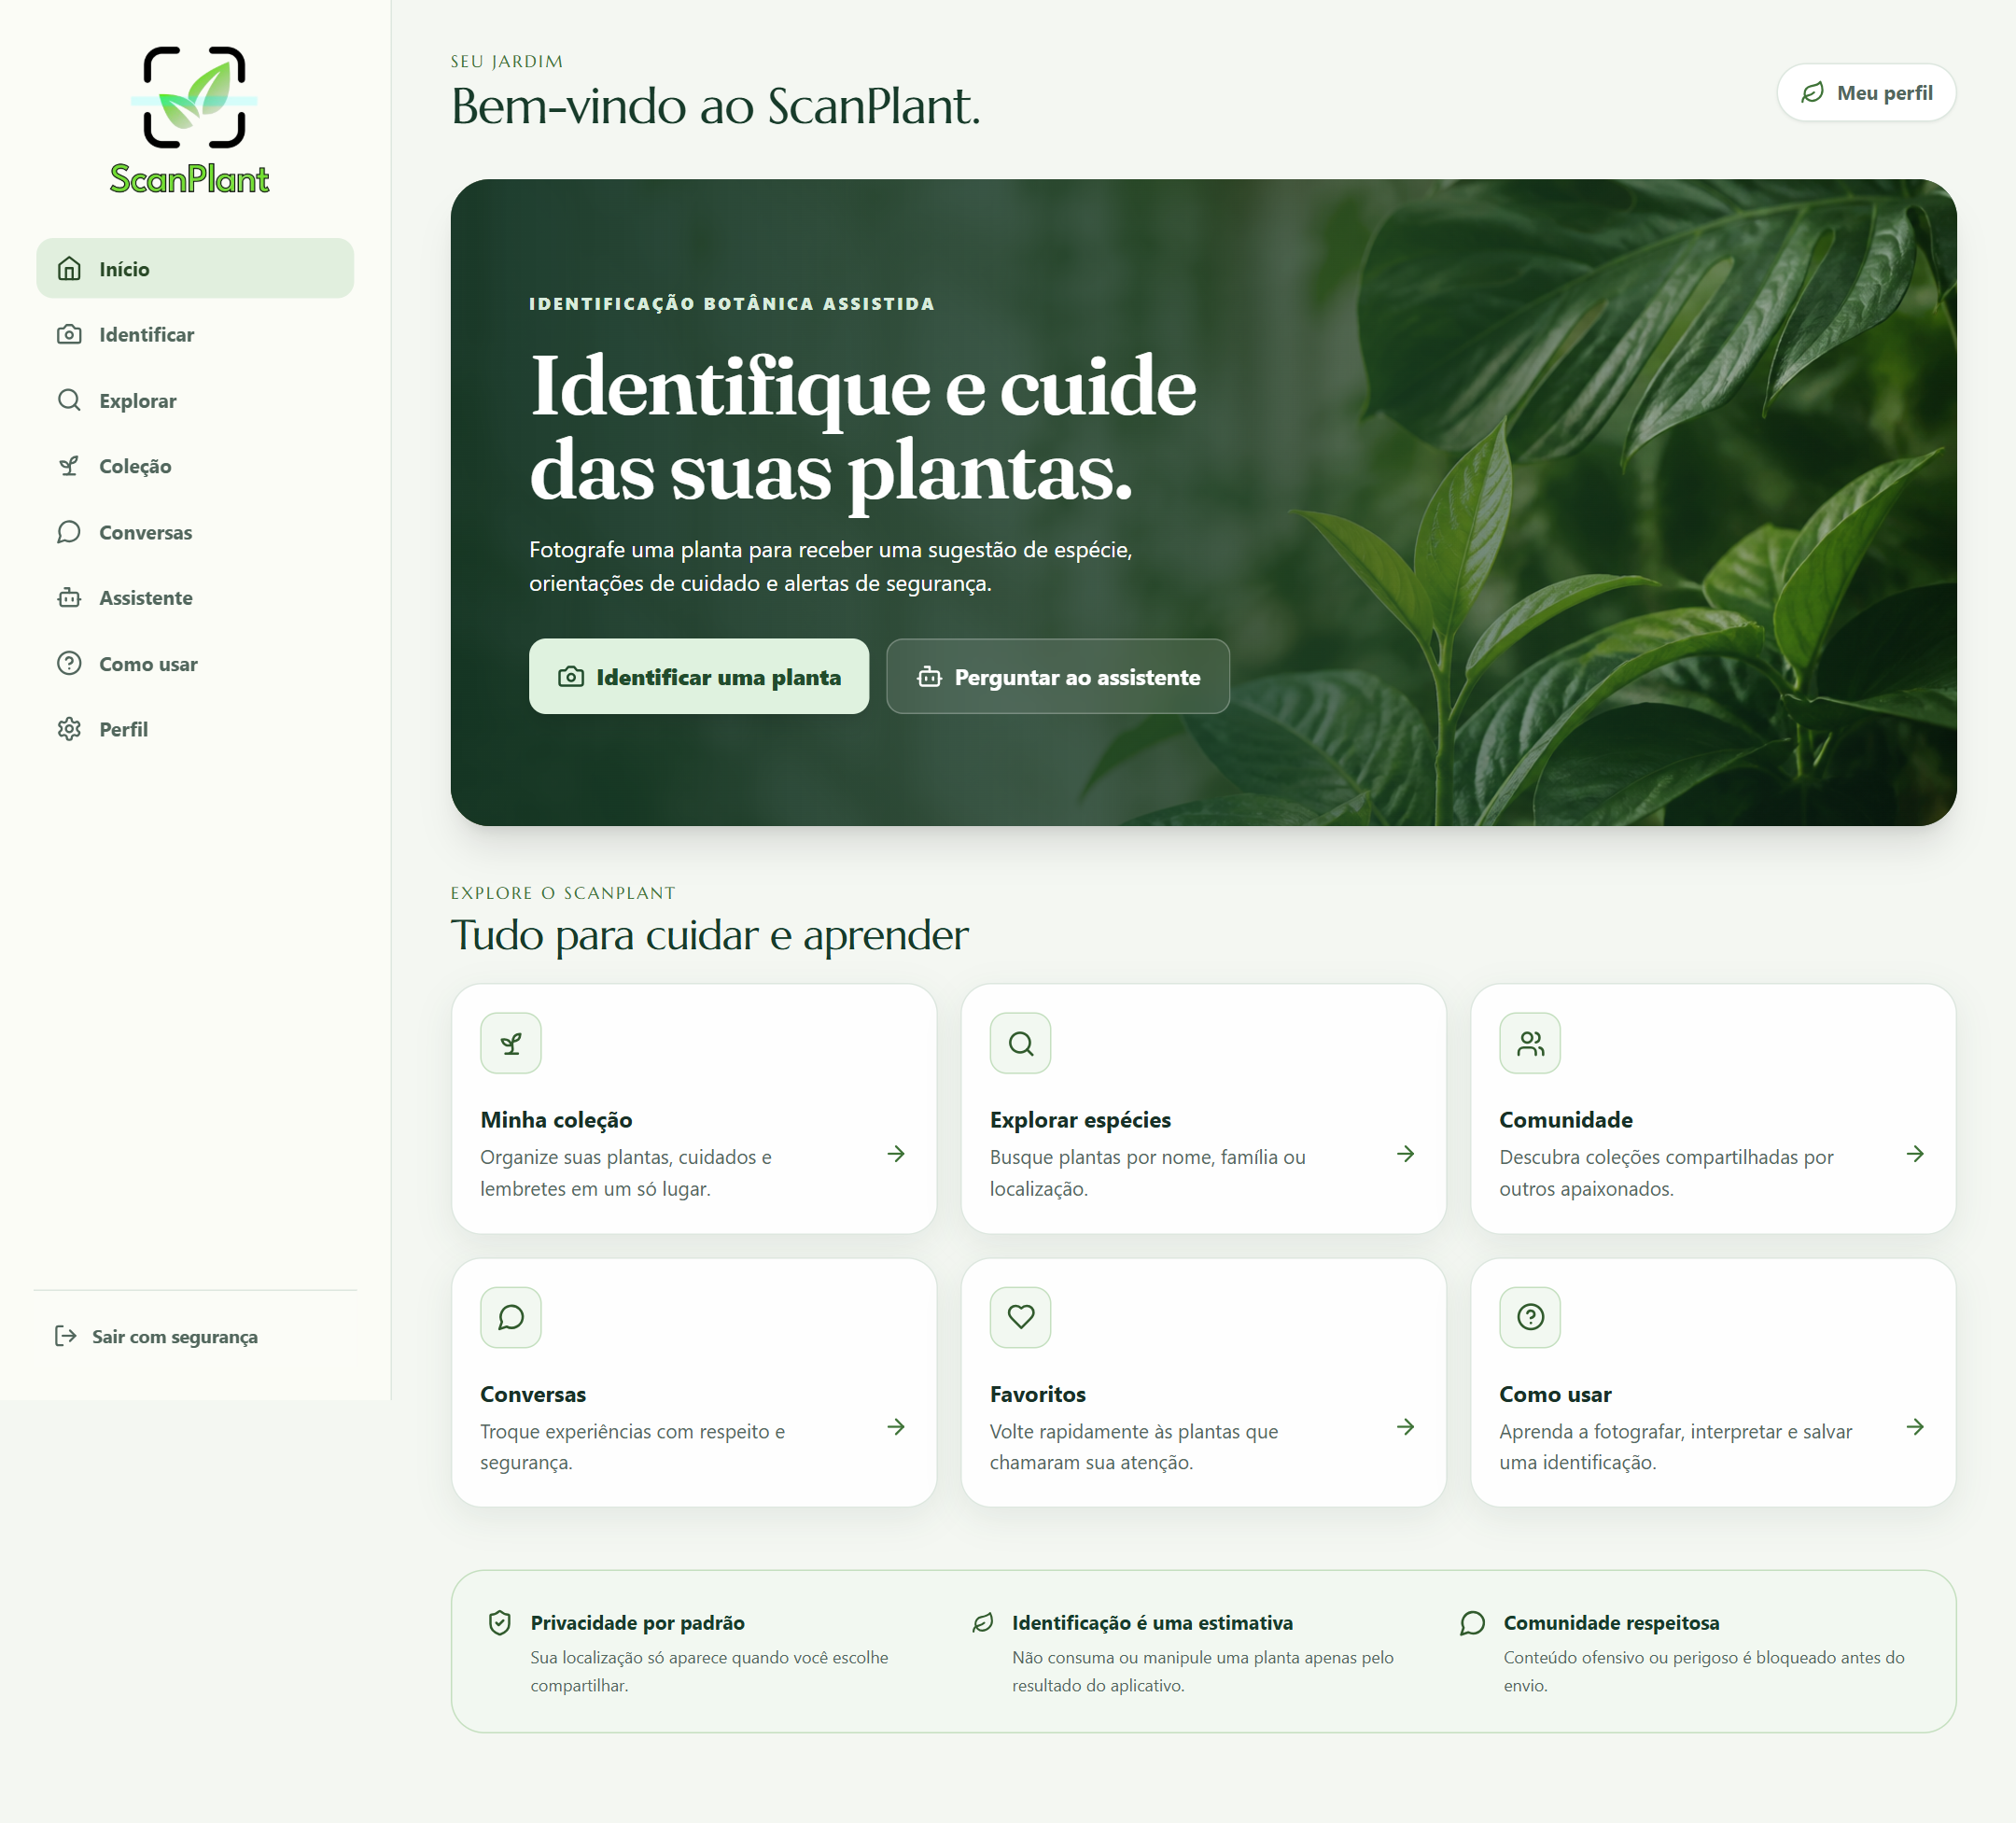
\includegraphics[width=0.80\textwidth]{figuras/sistema/figura10_dashboard.png}
\caption{Painel principal do ScanPlant após a autenticação}
\label{fig:dashboard}
\vspace{2pt}
\small
\noindent Fonte: Elaborada pelos autores a partir da versão publicada do ScanPlant (2026).
\end{figure}

O ScanPlant foi estruturado como uma plataforma integrada multiplataforma cujo fluxo de interação inicia-se na captura ou seleção de imagens foliares ou florais do espécime vegetal. A fotografia é submetida ao servidor por intermédio de endpoints RESTful autenticados, onde é processada pelo serviço de proxy. O back-end comunica-se com os modelos de visão computacional da API Plant.id, recuperando os nomes científico e popular da espécie, a família taxonômica e o percentual de acurácia estatística da predição.

A interface de identificação mostrada na Figura \ref{fig:identificacao} admite captura pela câmera ou envio de um arquivo já existente. Antes do processamento, o sistema apresenta orientações sobre enquadramento, iluminação e visibilidade da folha ou da flor. Também solicita a origem da fotografia e permite controlar sua exposição na comunidade. Esses campos articulam qualidade de entrada, rastreabilidade e privacidade: imagens nítidas favorecem a análise, enquanto a declaração de procedência e a escolha de compartilhamento tornam o uso posterior do registro mais transparente.

\begin{figure}[H]
\centering
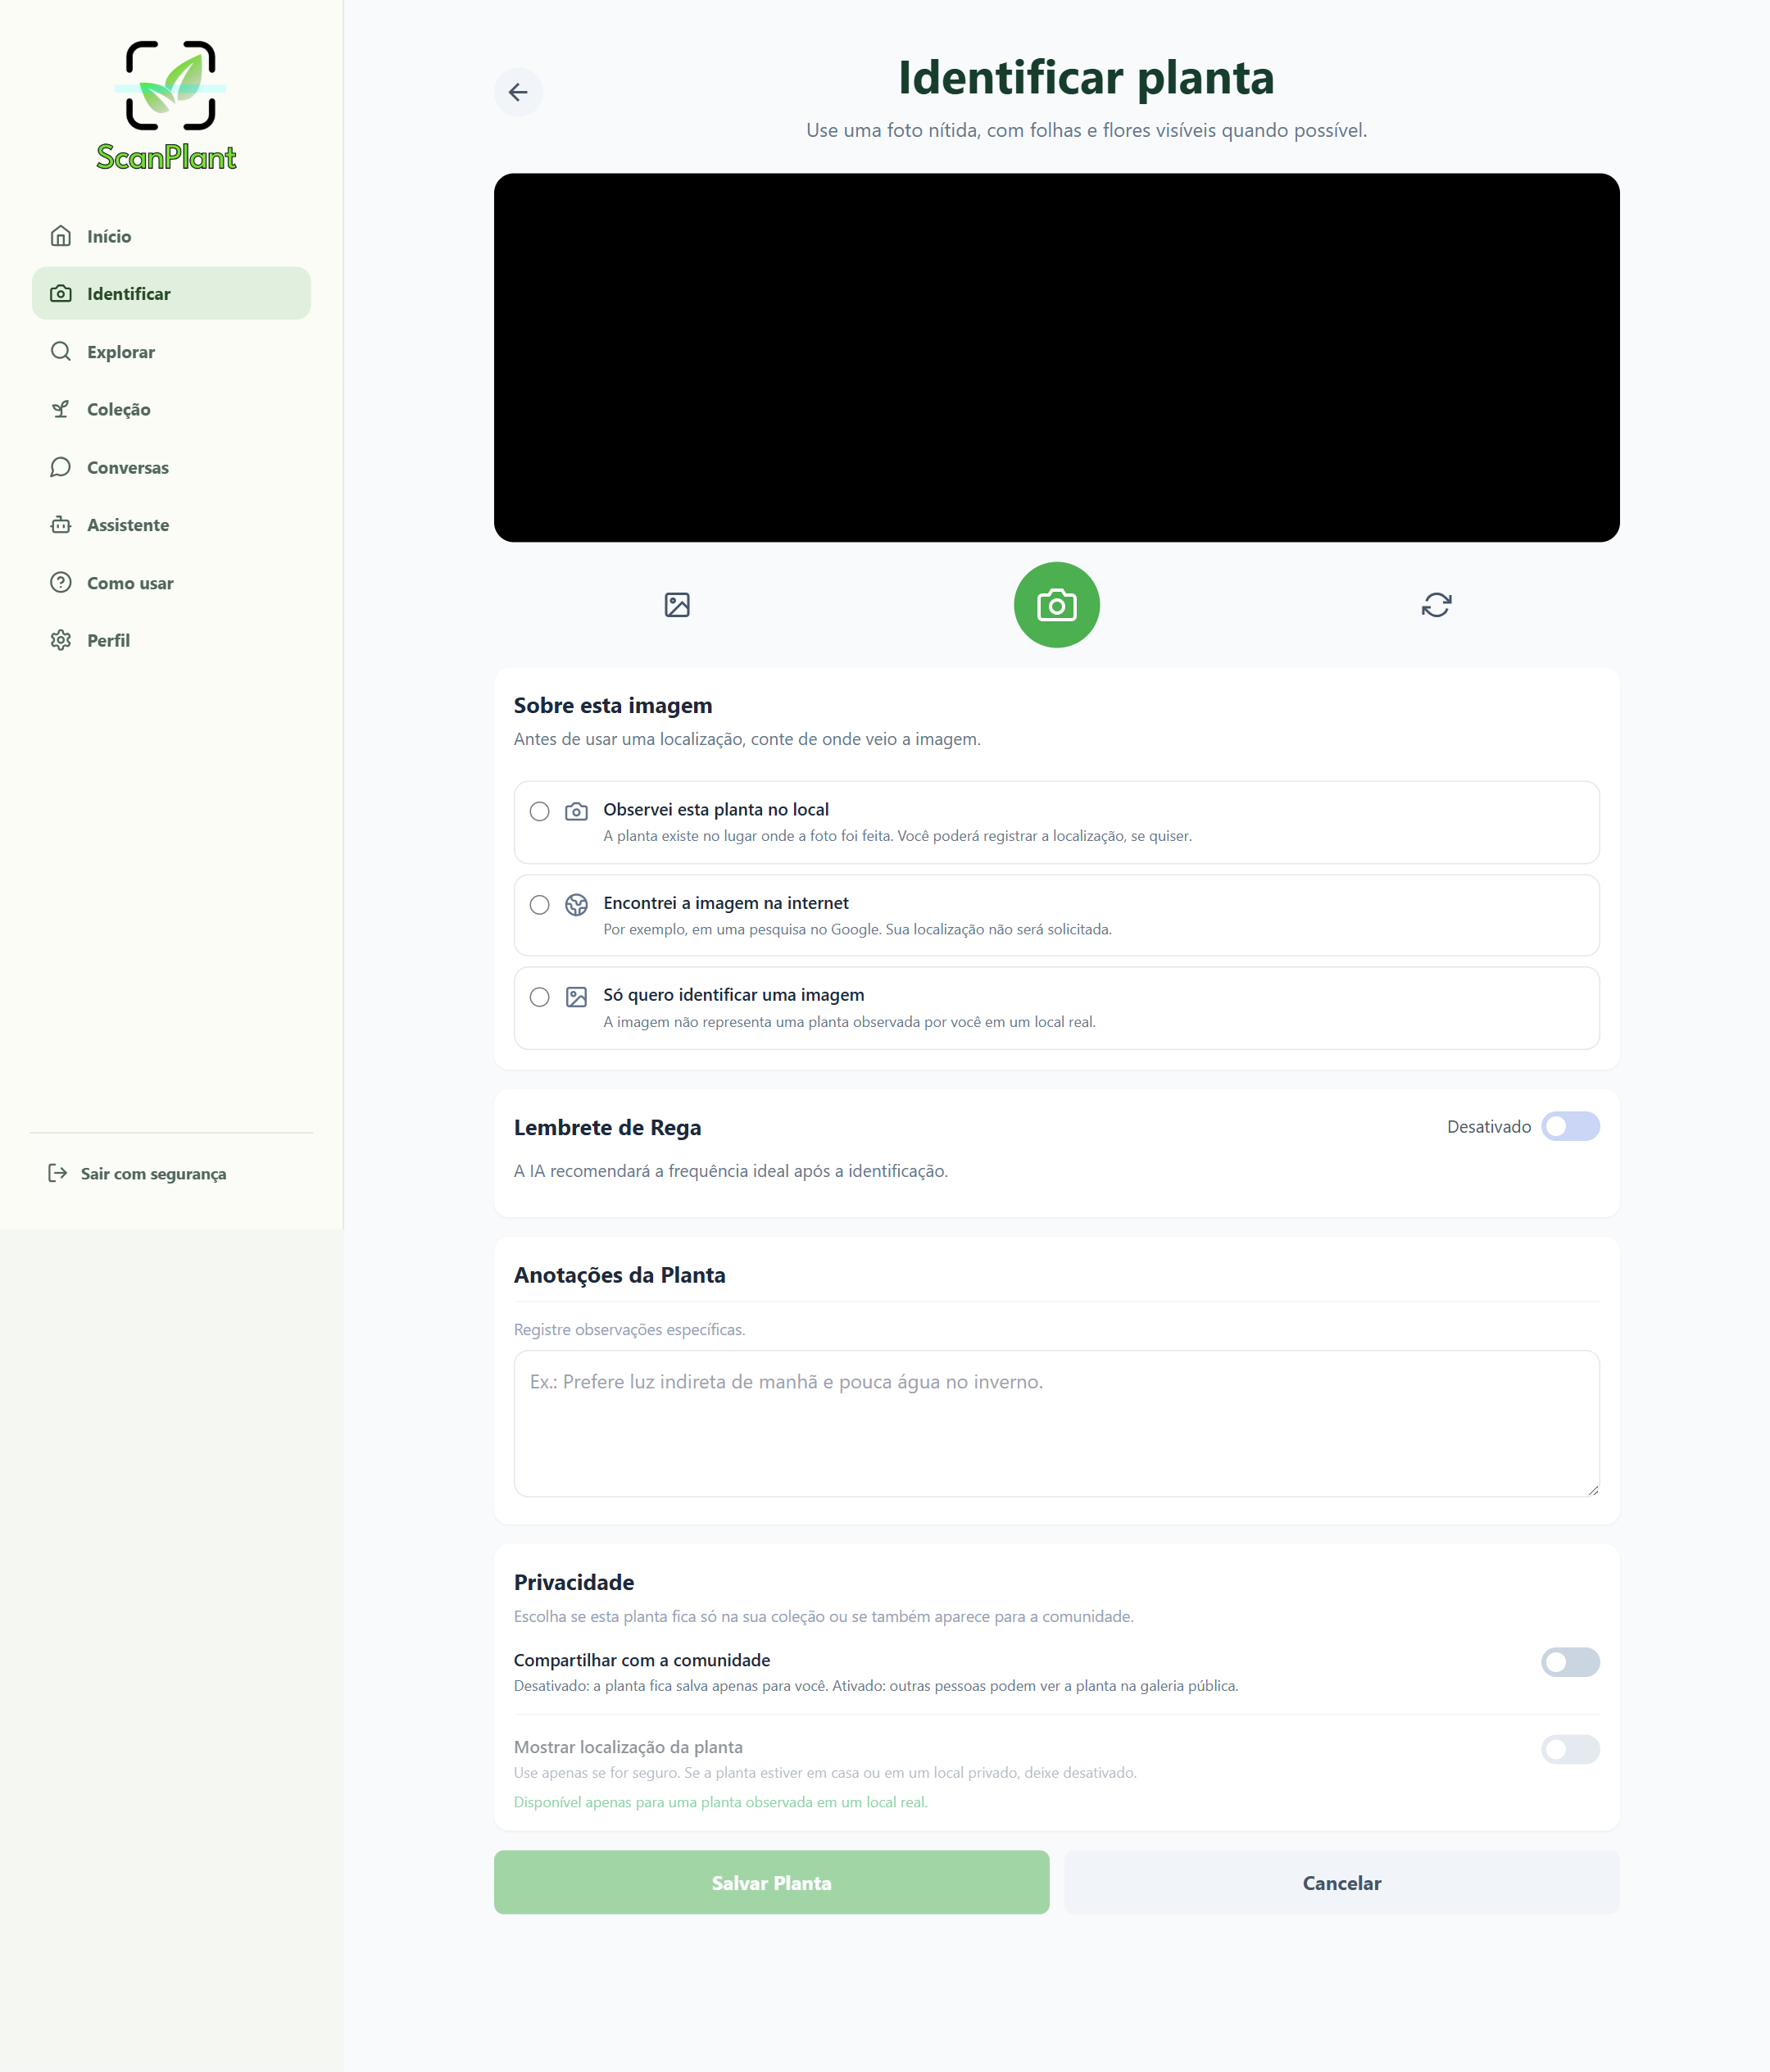
\includegraphics[width=0.74\textwidth]{figuras/sistema/figura11_identificacao.png}
\caption{Área de captura ou envio de fotografia para identificação botânica}
\label{fig:identificacao}
\vspace{2pt}
\small
\noindent Fonte: Elaborada pelos autores a partir da versão publicada do ScanPlant (2026).
\end{figure}

No ensaio, empregou-se uma fotografia de \textit{Monstera deliciosa} disponibilizada sob licença Creative Commons BY-SA, escolhida por apresentar uma folha em destaque e fenestrações visualmente características (Ramsey, 2006). O serviço retornou ``costela-de-adão'' e \textit{Monstera deliciosa}, com 86\% de correspondência. Conforme a Figura \ref{fig:resultado_identificacao}, a porcentagem é exibida ao lado da expressão ``resultado probabilístico'', o que fornece ao usuário uma medida de confiança sem ocultar a incerteza própria da classificação computacional.

\begin{figure}[H]
\centering
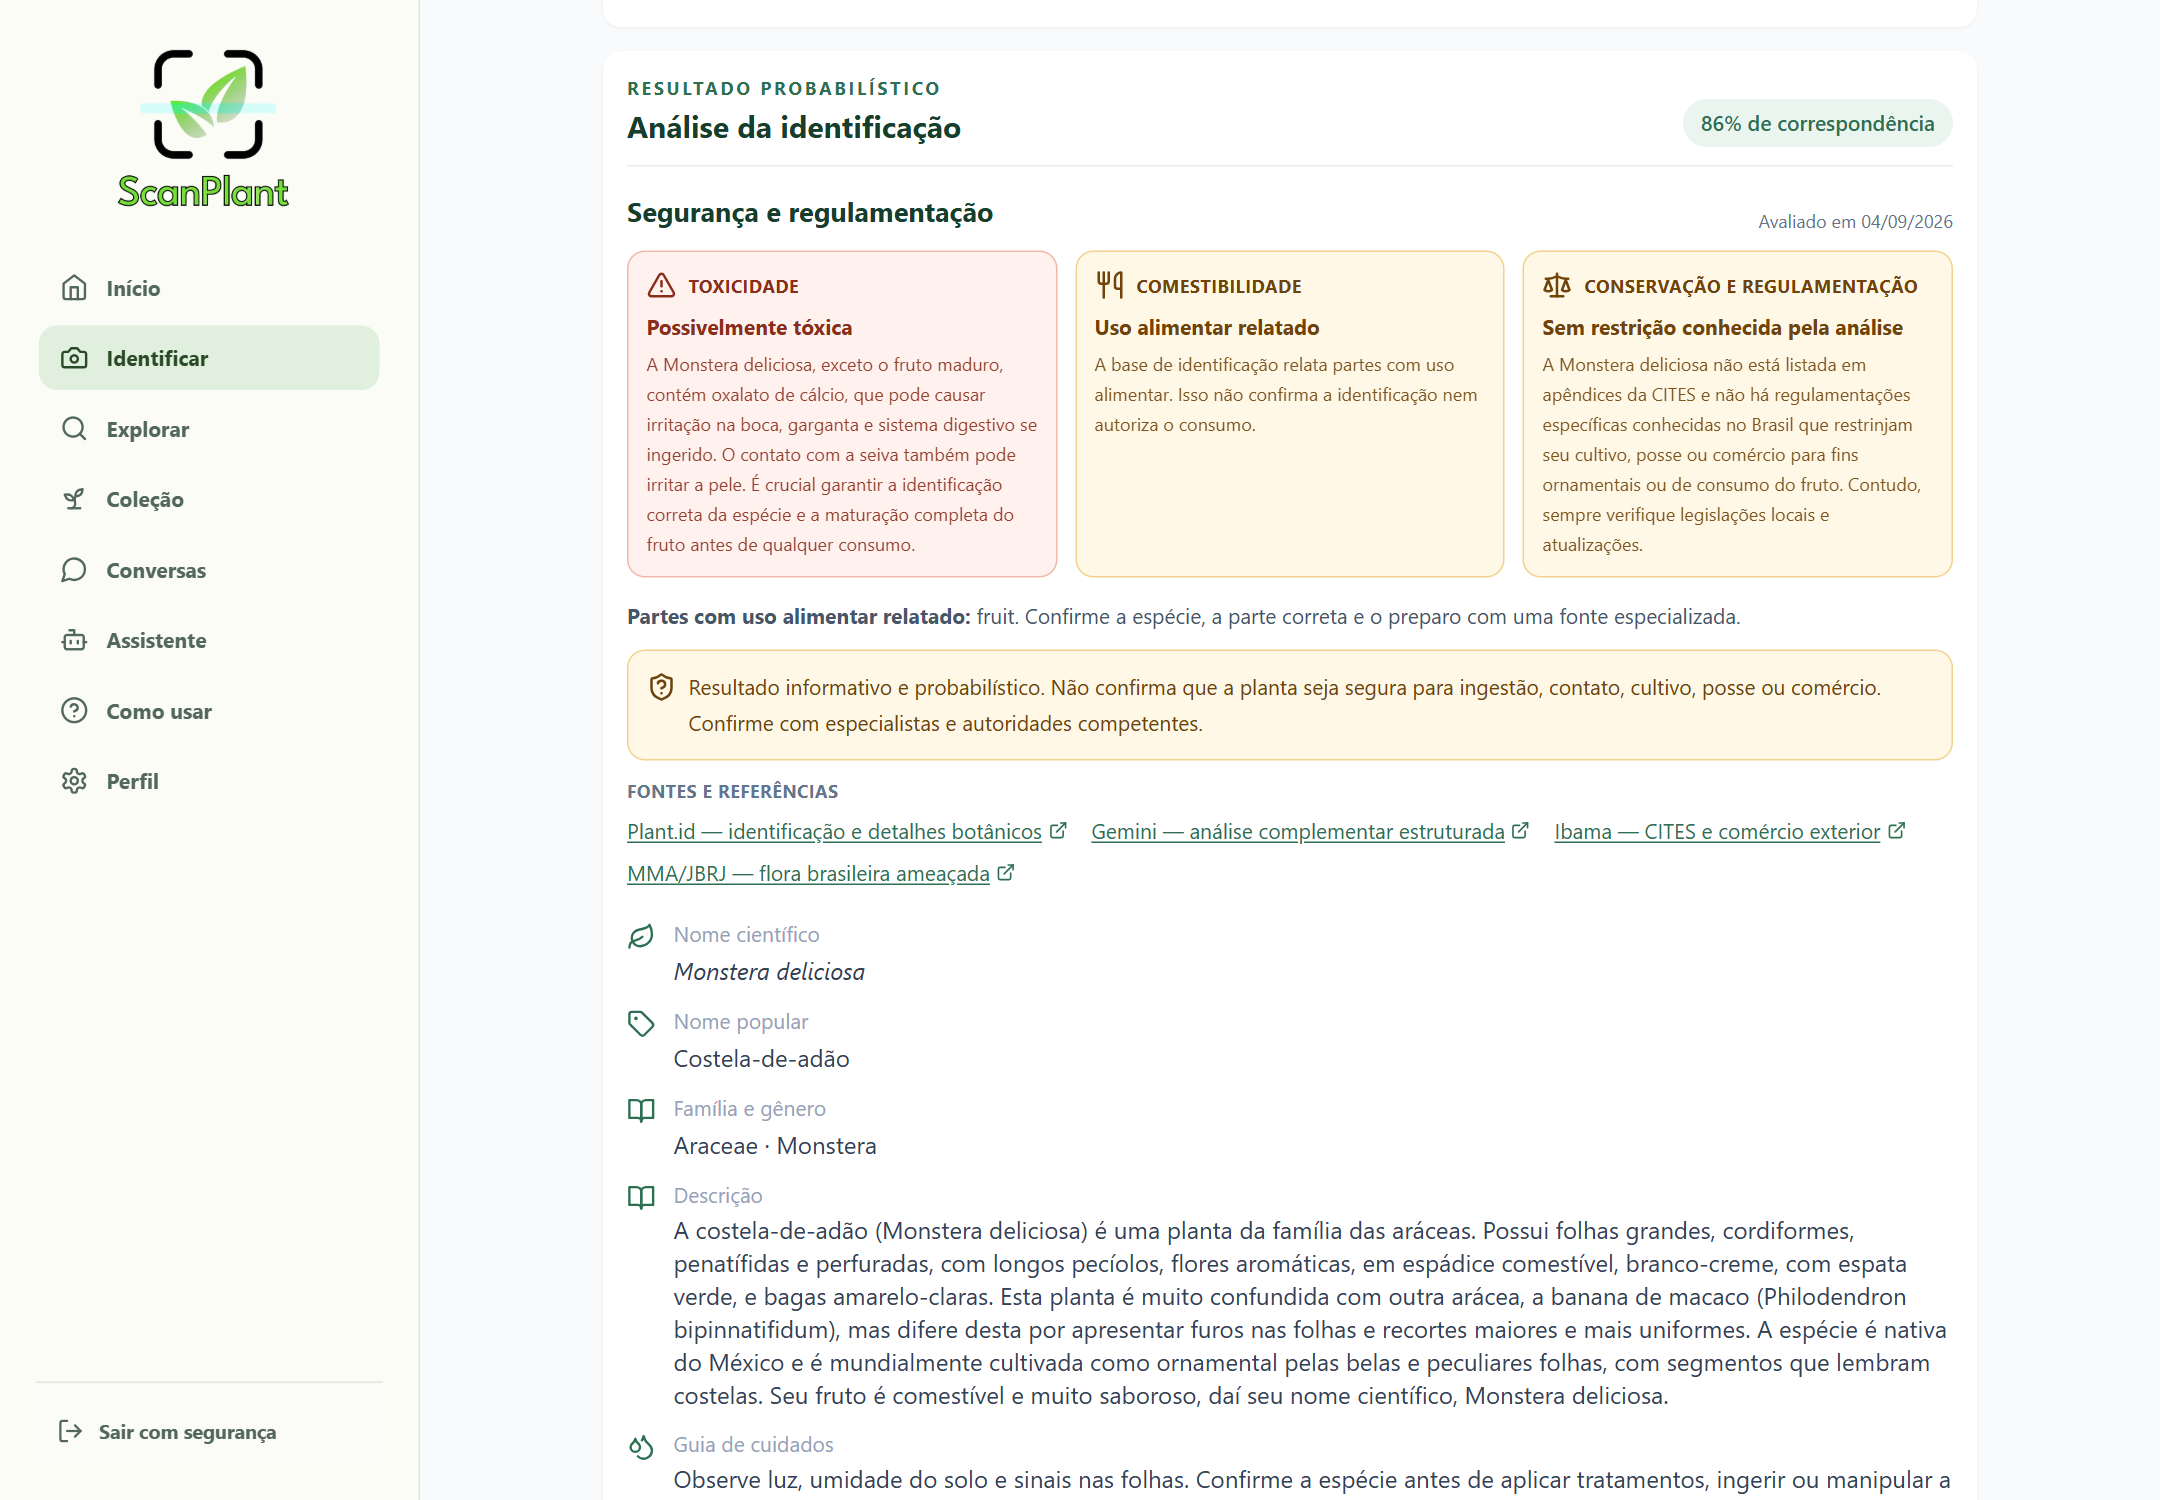
\includegraphics[width=0.96\textwidth]{figuras/sistema/figura12_resultado.png}
\caption{Resultado da identificação da costela-de-adão e síntese de segurança}
\label{fig:resultado_identificacao}
\vspace{2pt}
\small
\noindent Fonte: Elaborada pelos autores a partir da versão publicada do ScanPlant (2026), com fotografia de Ramsey (2006).
\end{figure}

Imediatamente após a identificação taxonômica, a resposta é submetida à camada interna de regras de negócio. Essa camada intercepta o resultado e consulta a base de segurança do sistema para verificar se a espécie apresenta compostos tóxicos para humanos ou animais domésticos, a exemplo de cristais de oxalato de cálcio (frequentes em Aráceas como a comigo-ninguém-pode e a costela-de-adão), saponinas hemolíticas ou alcaloides esteroidais (Botha; Penrith, 2008). Caso a planta seja catalogada como perigosa, a interface exibe um painel de alerta em destaque visual, contendo advertências claras de toxicidade e orientações de manuseio seguro.

O retorno obtido no teste separou três dimensões que poderiam ser confundidas pelo usuário: toxicidade, possibilidade de uso alimentar de partes específicas e situação de conservação ou regulamentação. A advertência sobre oxalato de cálcio foi apresentada em vermelho, enquanto a referência a uso alimentar permaneceu acompanhada da ressalva de que a identificação não autoriza o consumo. Além disso, a tela indicou as fontes externas utilizadas na composição do resultado. A combinação de cores, linguagem cautelar e rastreabilidade reduz o risco de uma leitura binária do tipo ``comestível ou tóxica'', especialmente em espécies cujo risco depende da parte da planta e do estado de maturação.

Após a identificação, o usuário pode adicionar a planta à sua coleção particular de cultivo. Nesse instante, o sistema aplica a regra de negócio para a criação de rotinas de irrigação: a partir do perfil hídrico cadastrado para a espécie, o ScanPlant calcula o intervalo médio recomendado entre regas e gera lembretes visuais periódicos. O cultivador tem a faculdade de confirmar o ato de rega por meio de um toque no botão correspondente, ação que atualiza o atributo de data da última rega e recalcula a data da próxima necessidade hídrica no banco de dados PostgreSQL.

Para verificar a persistência, a identificação foi salva com lembrete de rega a cada sete dias e uma anotação vinculada ao ensaio. A Figura \ref{fig:colecao_funcional} mostra que o item passou a integrar a coleção pessoal com nome popular, nome científico e indicação da periodicidade configurada. O resultado demonstra que a saída do módulo de reconhecimento não permanece isolada: ela se converte em um registro gerenciável e reutilizável no acompanhamento cotidiano.

\begin{figure}[H]
\centering
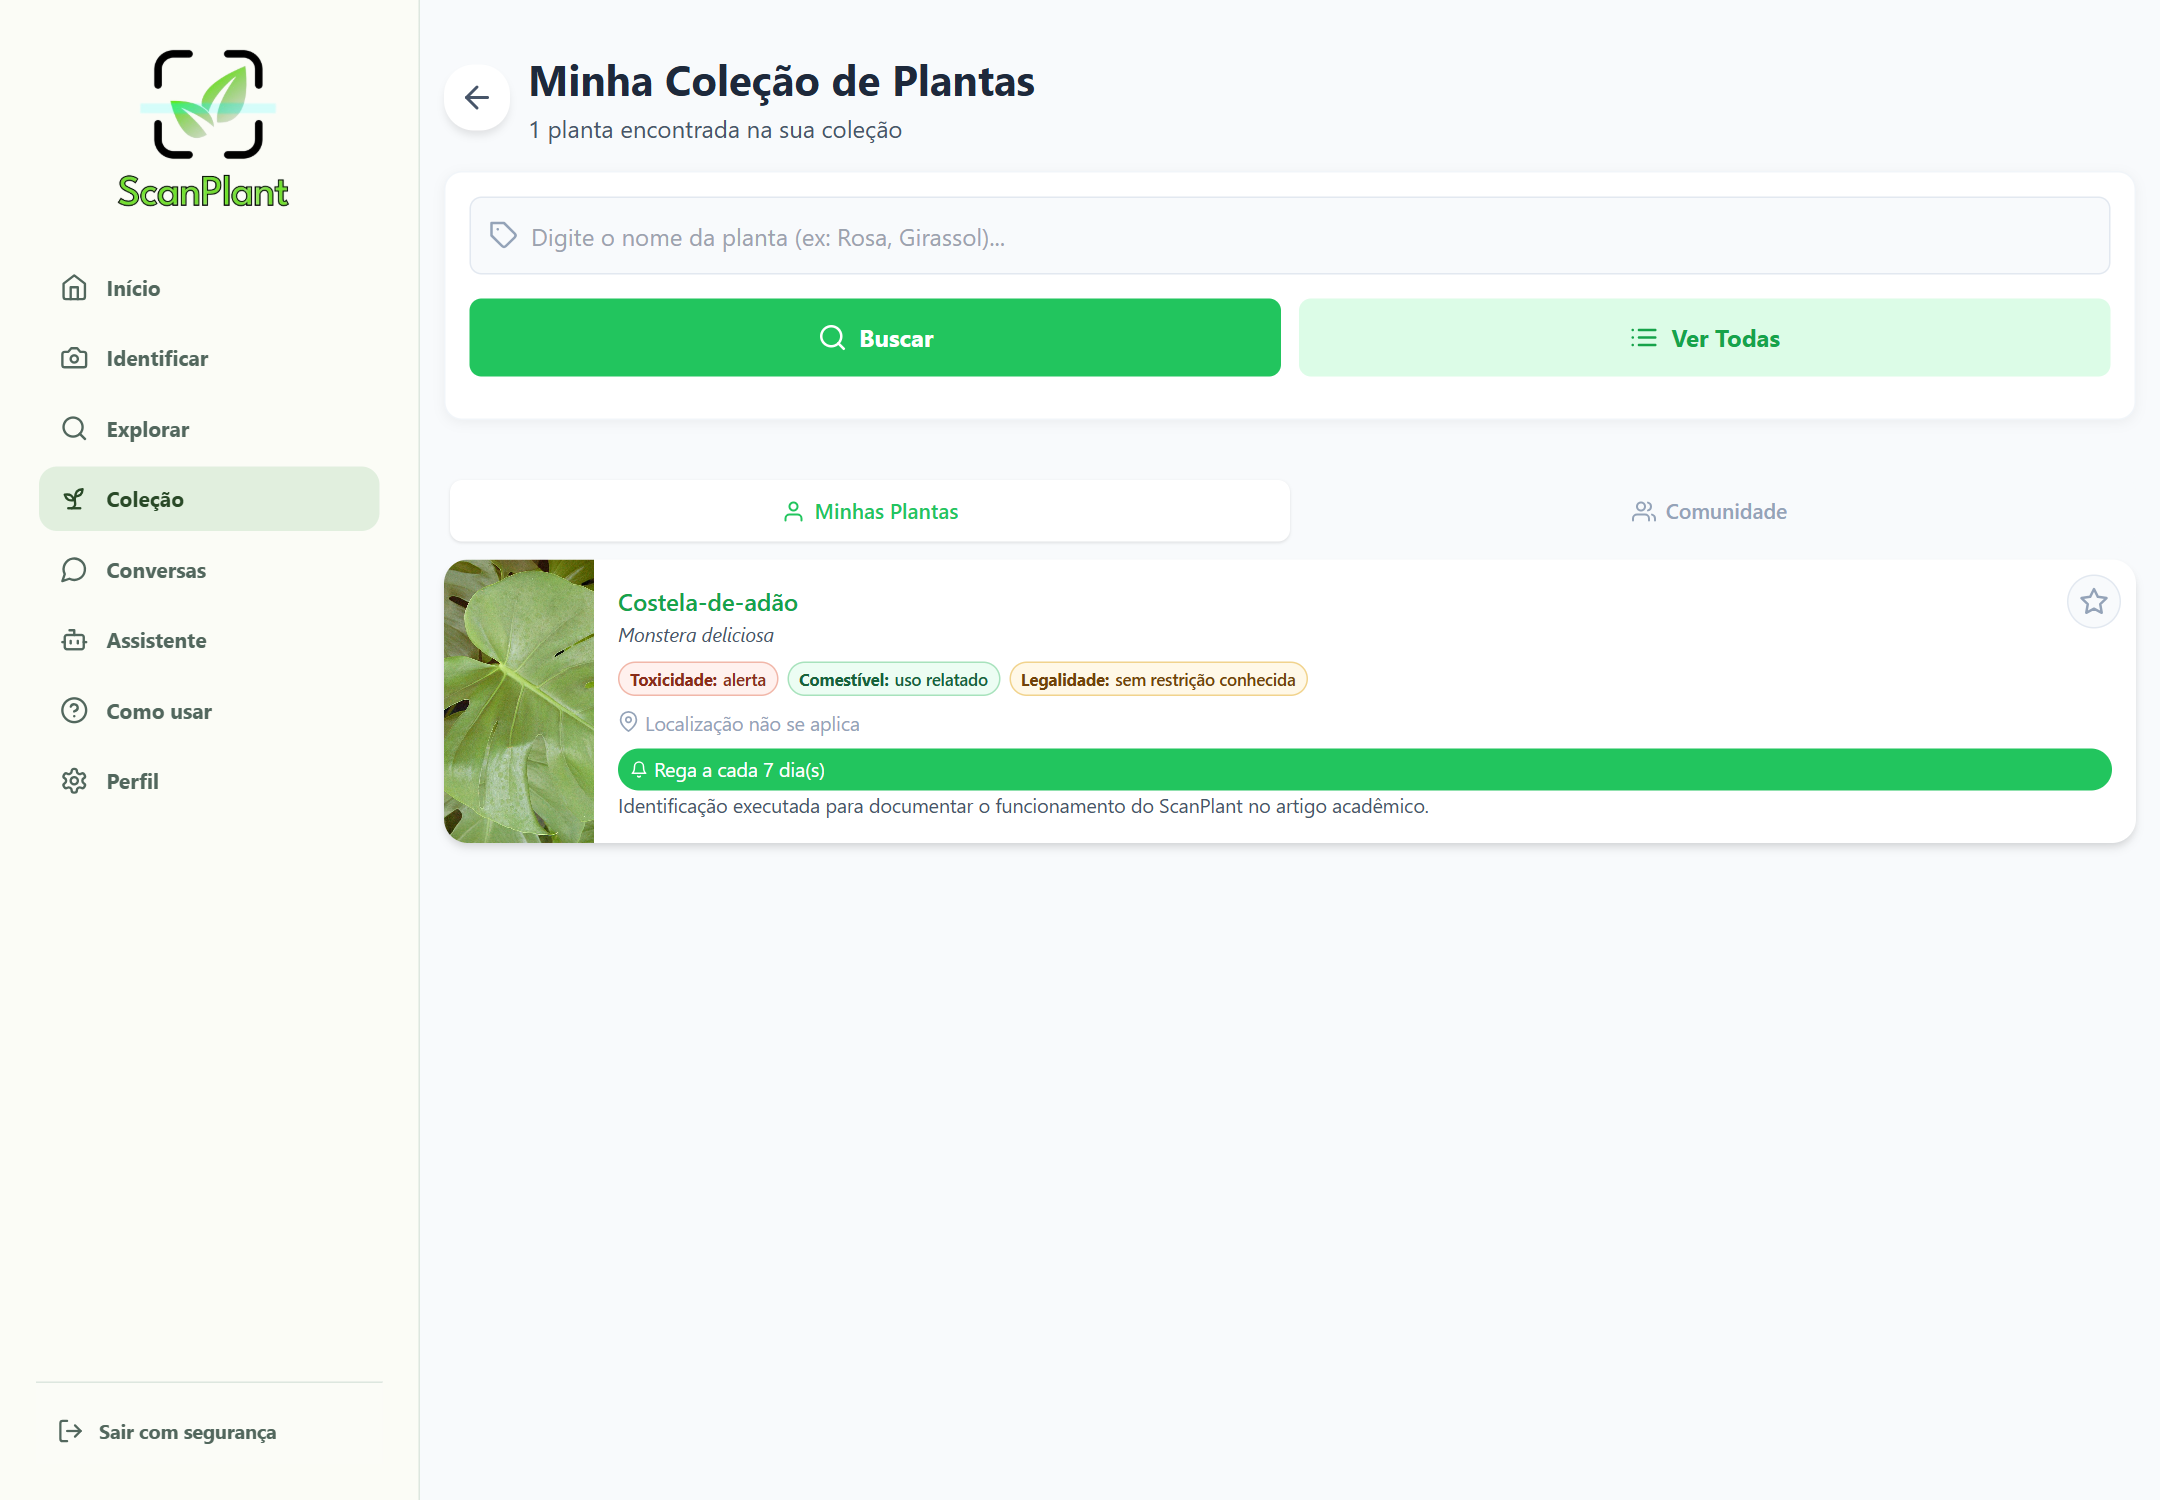
\includegraphics[width=0.90\textwidth]{figuras/sistema/figura13_colecao.png}
\caption{Coleção pessoal após o armazenamento da planta identificada}
\label{fig:colecao_funcional}
\vspace{2pt}
\small
\noindent Fonte: Elaborada pelos autores a partir da versão publicada do ScanPlant (2026).
\end{figure}

No que tange ao suporte conversacional, o usuário pode interagir diretamente com o assistente botânico movido por inteligência artificial generativa. No entanto, para coibir orientações médicas errôneas ou alucinações perigosas em situações de emergência, a aplicação implementa um pipeline de moderação com o serviço \texttt{ContentSafetyService}. Caso uma mensagem do usuário mencione sintomas de envenenamento, mastigação acidental de folhas por crianças ou ingestão por cães e gatos, o sistema bloqueia o despacho genérico ao LLM e aciona um protocolo de resposta prioritária de emergência, orientando o usuário a procurar assistência médica ou médico-veterinária imediata e disponibilizando canais diretos de contato com centros toxicológicos, como o SINITOX (FIOCRUZ).

No teste funcional, perguntou-se ao assistente como cuidar de uma costela-de-adão cultivada em ambiente interno. A resposta visível na Figura \ref{fig:assistente_funcional} organizou recomendações sobre luz indireta, intervalo de rega, umidade, substrato, adubação e suporte físico. A própria interface mantém um aviso para que o chat não seja usado como base única para decisões de ingestão ou uso medicinal. A resposta confirma o funcionamento do canal conversacional, mas sua formatação também revela uma oportunidade de melhoria: os marcadores de Markdown aparecem parcialmente como caracteres literais, tornando desejável aprimorar o renderizador de textos ricos para ampliar a legibilidade de respostas longas.

\begin{figure}[H]
\centering
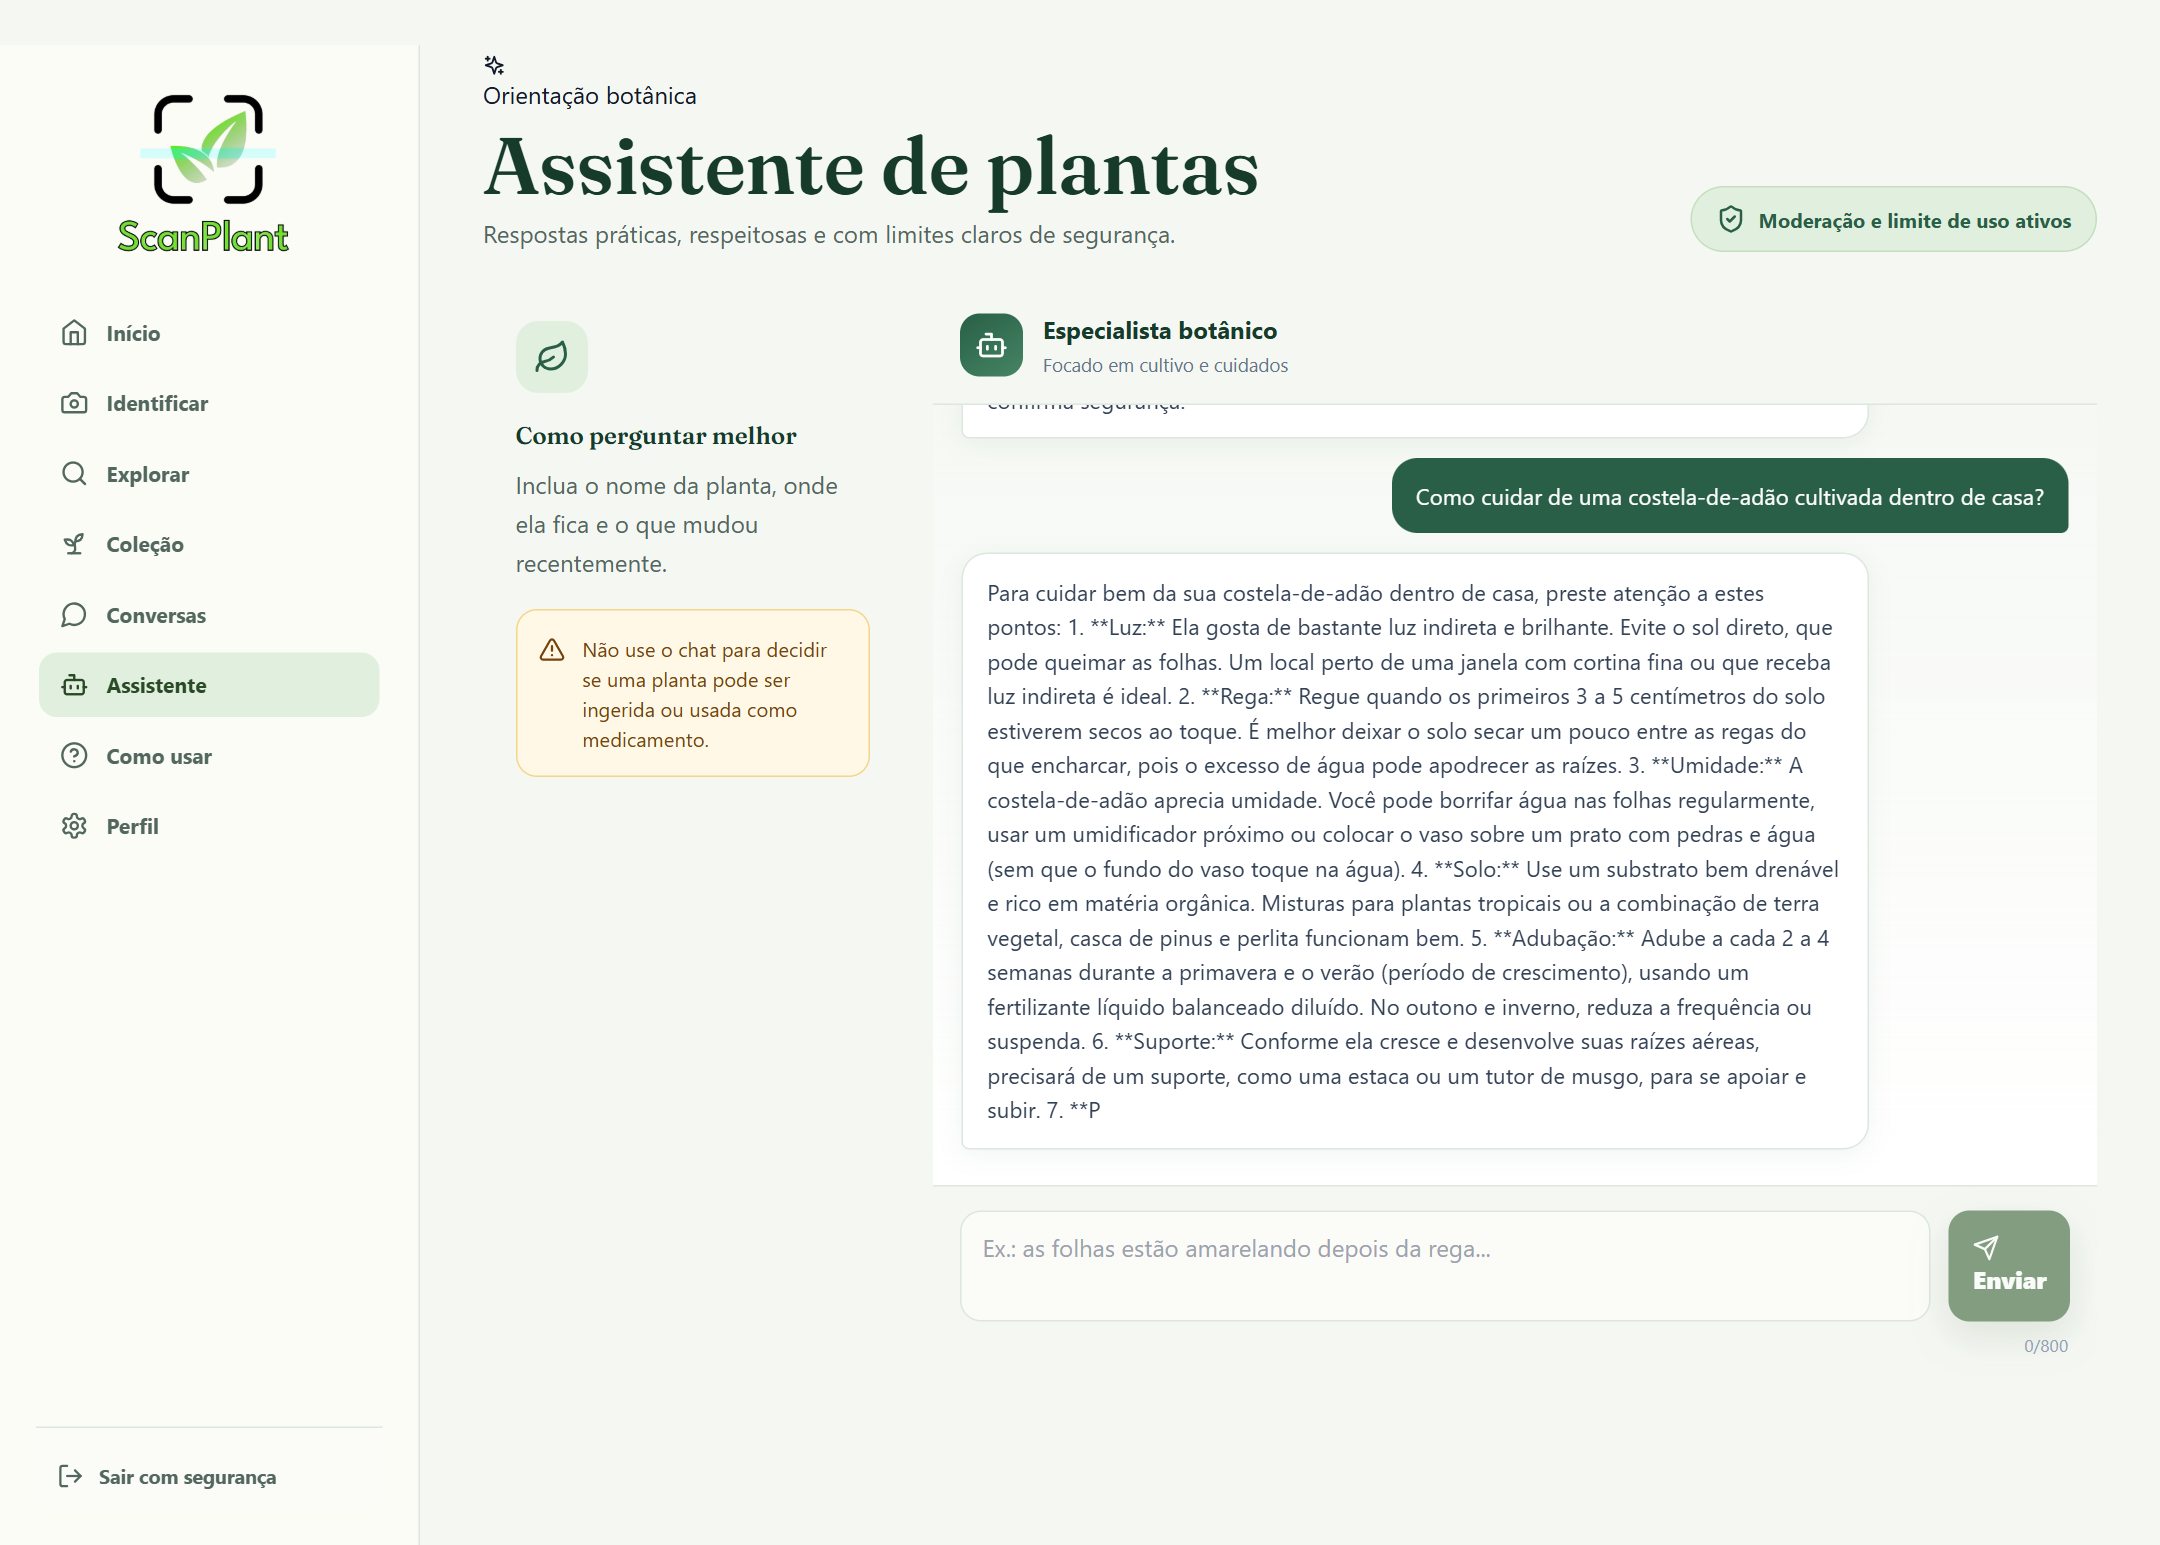
\includegraphics[width=0.96\textwidth]{figuras/sistema/figura15_assistente.png}
\caption{Assistente botânico respondendo a uma dúvida de cultivo}
\label{fig:assistente_funcional}
\vspace{2pt}
\small
\noindent Fonte: Elaborada pelos autores a partir da versão publicada do ScanPlant (2026).
\end{figure}

Em conjunto, as telas documentam um fluxo funcional de ponta a ponta, desde o acesso até a reutilização da identificação em uma consulta de cuidados. O ensaio não substitui testes de acurácia com uma amostra extensa de espécies, medições de desempenho ou avaliações formais de acessibilidade. Seu valor reside em demonstrar, com evidências reproduzíveis, que os componentes publicados trocam dados de modo coerente e que os mecanismos de cautela aparecem nos pontos de maior risco decisório. Essa delimitação evita extrapolar um caso bem-sucedido para conclusões universais sobre precisão botânica.

Por fim, o módulo de comunidade possibilita aos membros compartilhar imagens de seus exemplares e trocar experiências via chat. Para salvaguardar a integridade dos dados dos usuários conforme os princípios da Lei Geral de Proteção de Dados (LGPD), o sistema introduziu flags explícitas de controle de privacidade: o cultivador escolhe se a publicação deve ser pública ou restrita, e se suas coordenadas geográficas de localização devem ser exibidas, anonimizadas em nível municipal ou totalmente ocultadas.

\vspace{0.3cm}
\noindent \textbf{Síntese da Avaliação com Usuários}\par
\vspace{0.1cm}

A avaliação empírica foi realizada por meio de um questionário com 21 questões e 53 participantes ($N = 53$), combinando escalas de opinião, priorização de funcionalidades e campos abertos. A amostra foi composta majoritariamente por jovens de 18 a 25 anos (77,4\%); 81,1\% possuíam plantas em casa e 49,1\% se declararam iniciantes. Esses dados indicam proximidade com o público-alvo e, ao mesmo tempo, recomendam cautela na generalização dos resultados para outros perfis etários e níveis de experiência.

Antes da demonstração, a identificação por fotografia foi a funcionalidade mais priorizada, com 88,7\% de avaliações altas, seguida pelos lembretes de rega (84,9\%), alertas de toxicidade (83,0\%) e assistente conversacional (77,4\%). A preocupação elevada com plantas tóxicas foi registrada por 83,0\% dos respondentes. Quanto à privacidade, 43,4\% rejeitaram a divulgação irrestrita da localização exata e 35,8\% aceitariam o compartilhamento apenas mediante controle transparente, resultado que sustenta a adoção de configurações granulares de visibilidade.

A Figura \ref{fig:sintese_avaliacao} reúne os indicadores posteriores à apresentação da plataforma. A impressão geral foi positiva ou muito positiva para 94,3\% dos participantes; 90,5\% classificaram o design como agradável ou muito agradável e a mesma proporção considerou o uso fácil ou muito fácil. A clareza do processo de identificação obteve 92,4\% de avaliações favoráveis. Na escala de utilidade, o sistema alcançou média de 8,91 em 10, enquanto o Net Promoter Score resultou em +71,7, com 75,5\% de promotores e 3,8\% de detratores.

\begin{figure}[H]
\centering
\begin{subfigure}[t]{0.82\textwidth}
  \centering
  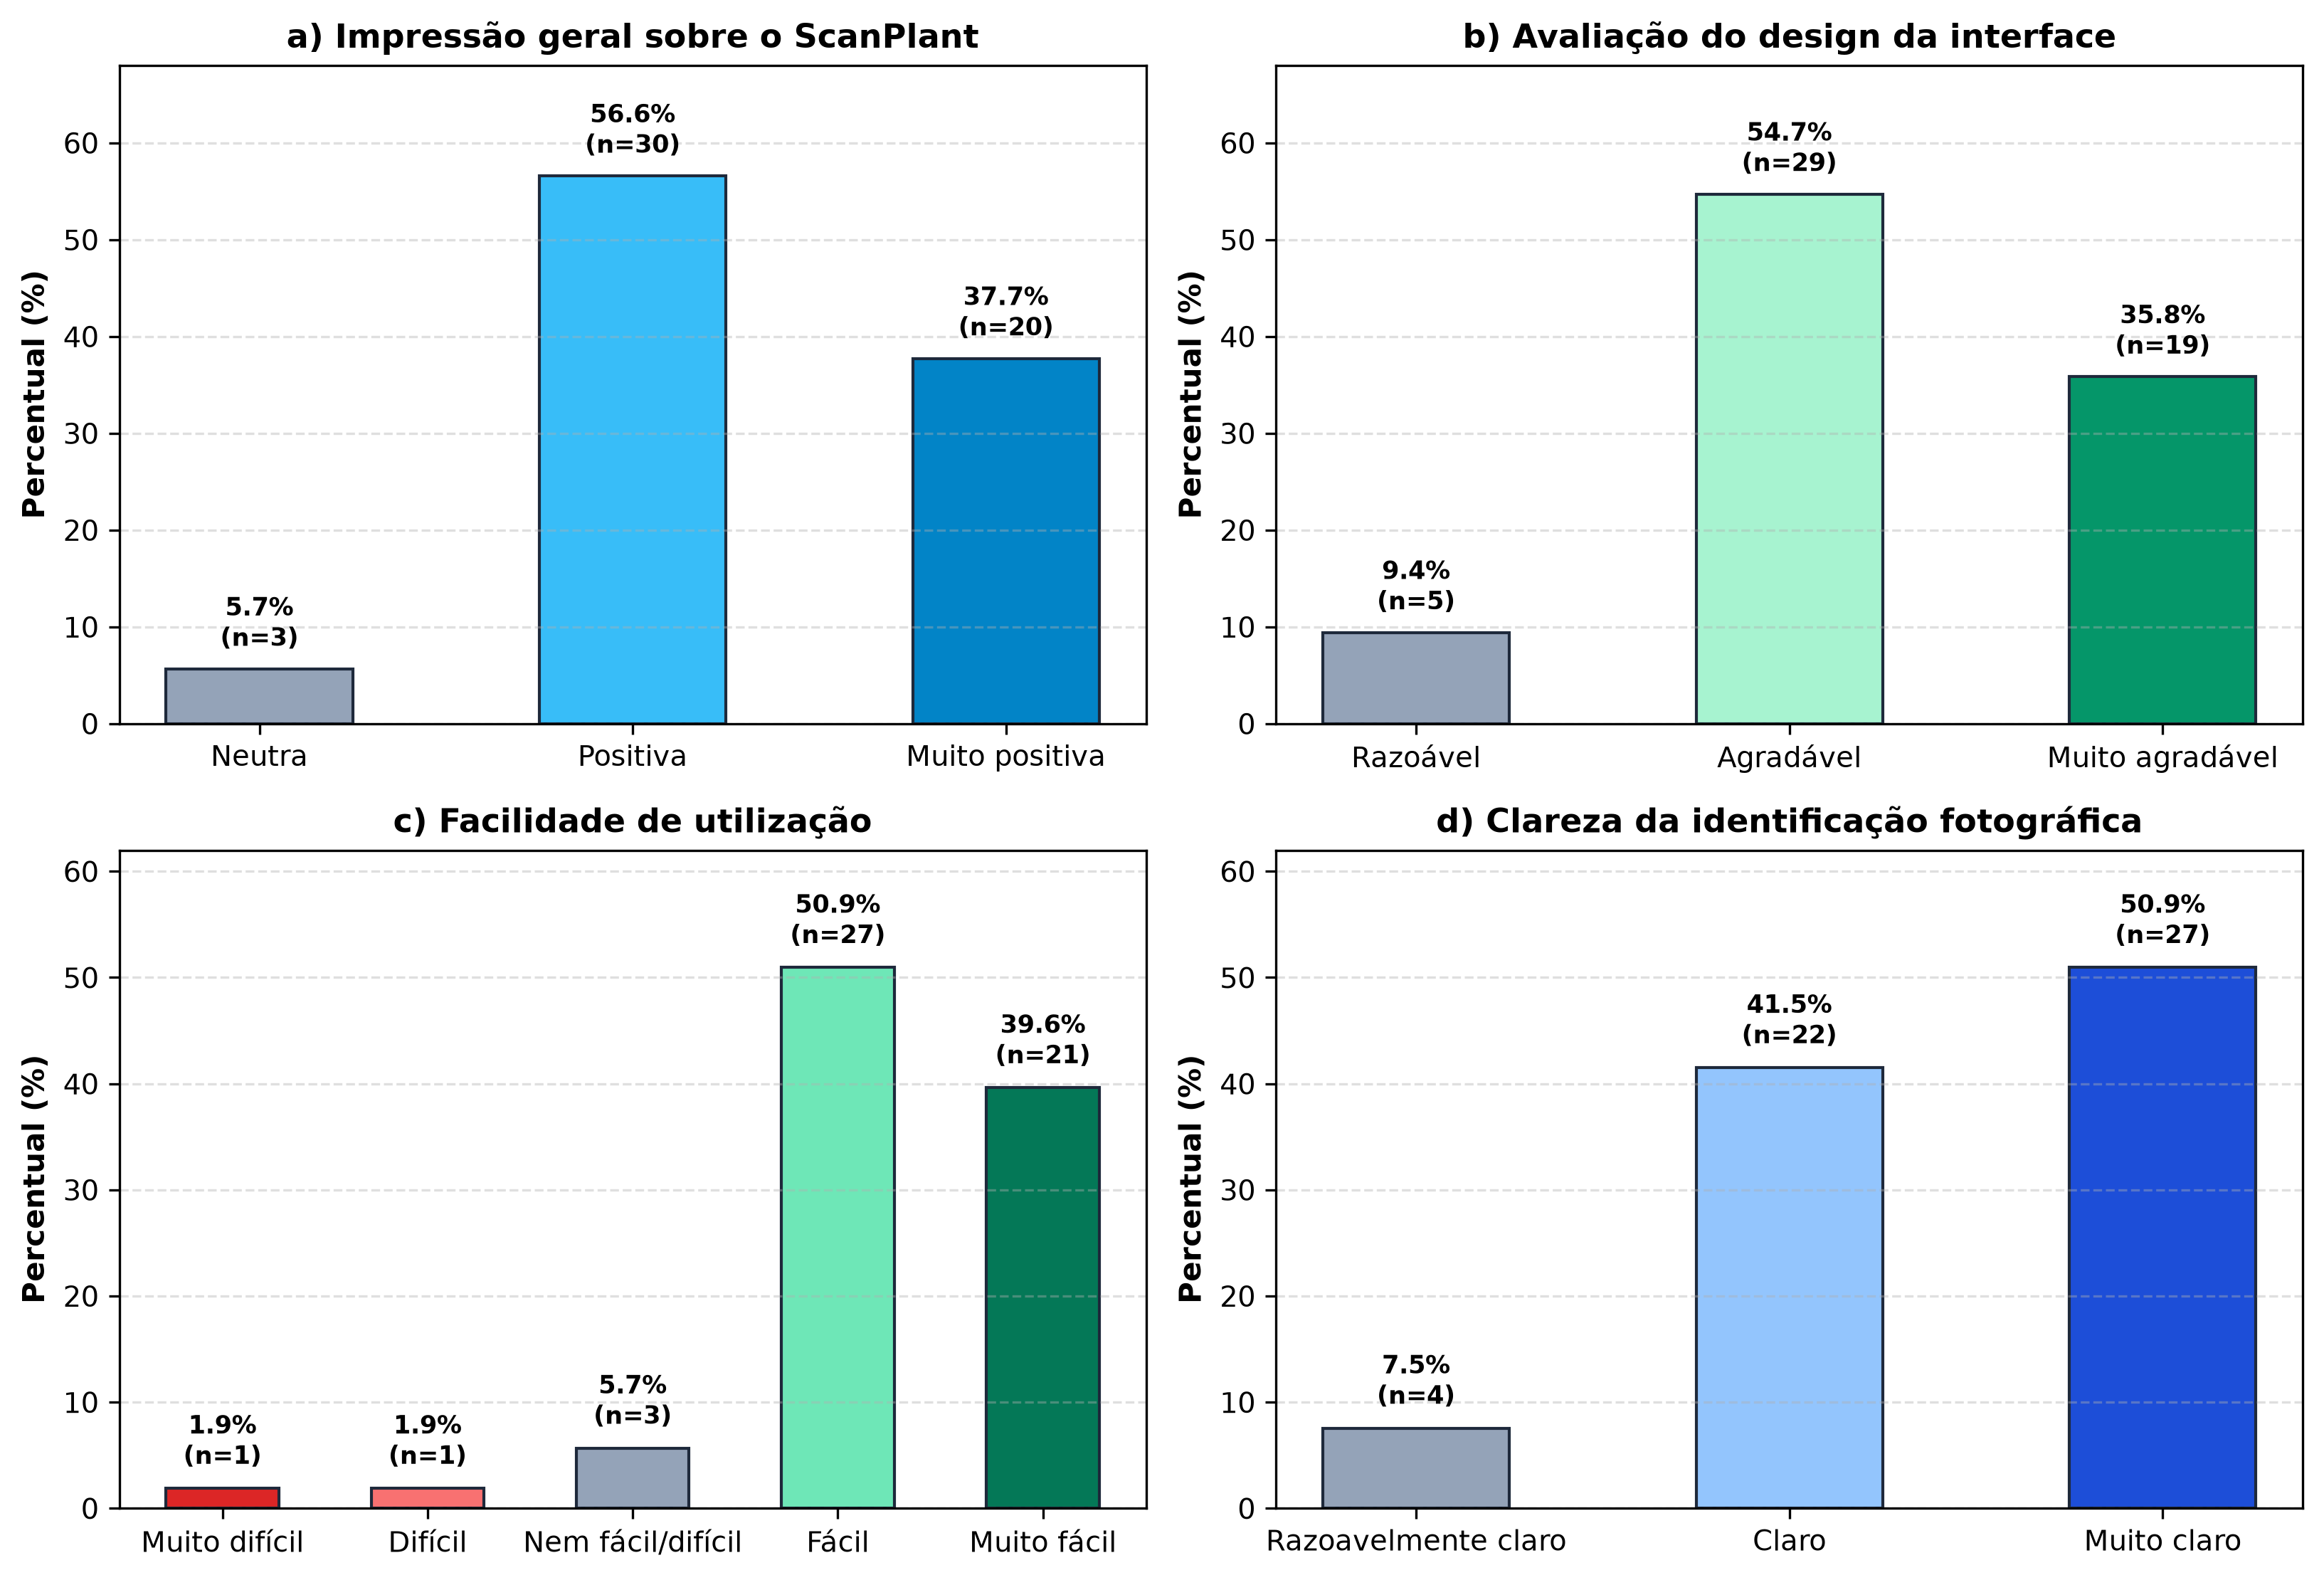
\includegraphics[width=\textwidth]{figuras/grafico6_avaliacao_pos_demo.png}
  \caption{Percepção da interface e da identificação após a demonstração}
\end{subfigure}

\vspace{0.2cm}
\begin{subfigure}[t]{0.82\textwidth}
  \centering
  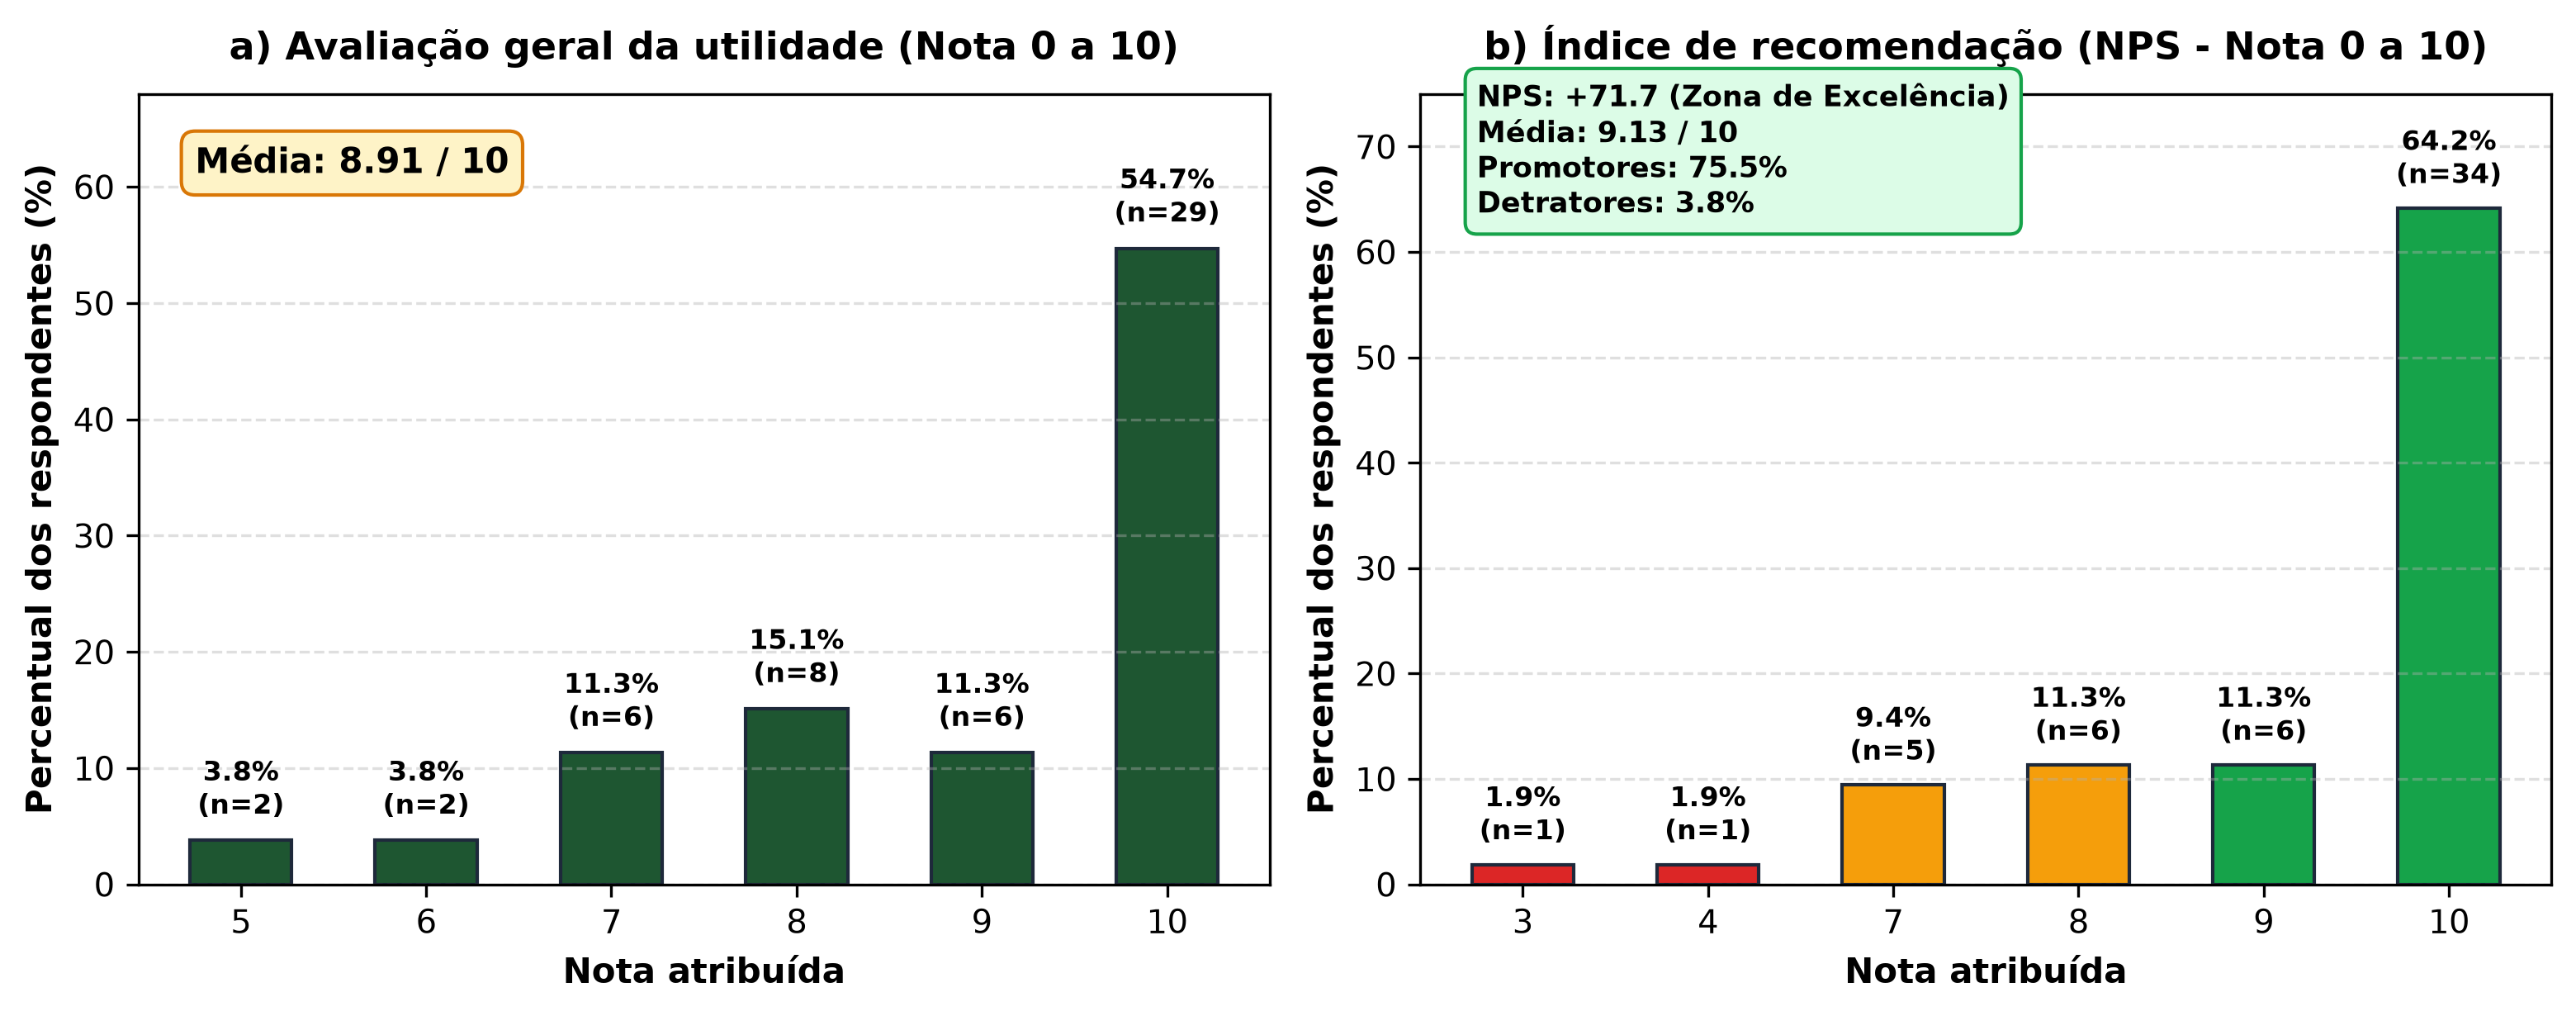
\includegraphics[width=\textwidth]{figuras/grafico7_nps_utilidade.png}
  \caption{Utilidade percebida e índice de recomendação}
\end{subfigure}
\caption{Síntese dos resultados da avaliação do ScanPlant ($N = 53$)}
\label{fig:sintese_avaliacao}
\vspace{2pt}
\small
\noindent Fonte: Elaborada pelos autores com base nos dados da pesquisa.
\end{figure}

As respostas abertas concentraram-se em dificuldades de rega, luminosidade, nutrição do solo, pragas e segurança de animais domésticos. Entre as melhorias sugeridas destacaram-se a formatação mais clara das respostas do assistente, o histórico fotográfico das plantas, a organização da coleção por ambientes e a consulta offline de informações básicas. Esses achados são coerentes com as funções já implementadas e oferecem prioridades objetivas para versões futuras, sem substituir testes controlados de precisão, desempenho e acessibilidade.

Em conjunto, a demonstração funcional e a avaliação com usuários indicam que a integração entre identificação, alertas, coleção e assistência conversacional responde a necessidades práticas do cultivo doméstico. A interpretação deve permanecer proporcional ao desenho do estudo: os resultados demonstram aceitação e funcionamento em um cenário específico, mas não constituem comprovação universal de acurácia botânica.

% ==============================================================================
% 5 CONSIDERAÇÕES FINAIS
% ==============================================================================
\section{CONSIDERAÇÕES FINAIS}

Este trabalho apresentou o desenvolvimento e a avaliação do ScanPlant, plataforma que integra identificação botânica por imagem, alertas de segurança, organização de coleções, lembretes e assistência conversacional. A arquitetura em C\# (.NET 8), PostgreSQL, React e React Native permitiu separar as responsabilidades do sistema e conectar as interfaces aos serviços externos de inteligência artificial por meio de uma camada servidora controlada.

A demonstração da versão web publicada confirmou o percurso entre autenticação, envio da fotografia, retorno probabilístico, armazenamento da planta e consulta ao assistente. No cenário testado, uma fotografia de \textit{Monstera deliciosa} foi reconhecida com 86\% de correspondência e acompanhada por advertências de toxicidade, uso alimentar e regulamentação. As telas também evidenciaram que o sistema comunica a incerteza da classificação e orienta a confirmação com fontes especializadas.

A avaliação com 53 participantes registrou média de utilidade de 8,91 em 10 e NPS de +71,7. Os resultados sustentam a relevância das funções centrais, mas devem ser interpretados dentro dos limites da amostra e do caráter demonstrativo do estudo. A contribuição do projeto reside sobretudo na reunião de recursos que normalmente aparecem fragmentados, com atenção à privacidade e à prevenção de decisões inseguras.

Permanecem como limitações a dependência de conexão com a internet, a necessidade de ampliar os testes com diferentes espécies e condições fotográficas e a apresentação ainda simples de respostas longas do assistente. Como continuidade, recomendam-se um histórico fotográfico por planta, organização da coleção por ambientes, aperfeiçoamento do conteúdo formatado, avaliação formal de acessibilidade e recursos básicos de consulta offline.

Conclui-se que o ScanPlant constitui uma aplicação funcional e pertinente ao cultivo doméstico, ao aproximar visão computacional, modelos generativos e práticas de engenharia de software. Seu uso, contudo, deve permanecer informativo e complementar ao conhecimento de especialistas, especialmente em decisões relacionadas à ingestão, toxicidade e manejo de espécies potencialmente perigosas.

% ==============================================================================
% BARREIRA DE FLUTUAÇÃO: IMPEDE QUE ELEMENTOS FLUTUEM PARA AS REFERÊNCIAS
% ==============================================================================
\FloatBarrier

% ==============================================================================
% REFERÊNCIAS
% ==============================================================================
\section*{REFERÊNCIAS}
\addcontentsline{toc}{section}{REFERÊNCIAS}

\noindent BOOCH, G.; RUMBAUGH, J.; JACOBSON, I. \textbf{UML: guia do usuário}. 2. ed. Rio de Janeiro: Elsevier, 2006.

\vspace{0.2cm}
\noindent BOTHA, C. J.; PENRITH, M. L. Potential plant poisonings in domestic animals in South Africa. \textbf{Journal of the South African Veterinary Association}, v. 79, n. 4, p. 166--174, 2008.

\vspace{0.2cm}
\noindent FLORA INCOGNITA. \textbf{Flora Incognita: automated plant species identification}. Technische Universität Ilmenau e Max Planck Institute, 2024. Disponível em: \url{https://floraincognita.com/}. Acesso em: 15 out. 2024.

\vspace{0.2cm}
\noindent GIL, A. C. \textbf{Como elaborar projetos de pesquisa}. 6. ed. São Paulo: Atlas, 2019.

\vspace{0.2cm}
\noindent GOËAU, H.; BONNET, P.; JOLY, A. Overview of LifeCLEF Plant Identification Task 2018. In: \textbf{CLEF (Working Notes)}, 2018.

\vspace{0.2cm}
\noindent GOODFELLOW, I.; BENGIO, Y.; COURVILLE, A. \textbf{Deep learning}. Cambridge: MIT Press, 2016.

\vspace{0.2cm}
\noindent GOOGLE. \textbf{Google Gemini API Documentation: build with generative AI models}. 2024. Disponível em: \url{https://ai.google.dev/}. Acesso em: 20 out. 2024.

\vspace{0.2cm}
\noindent HALL, C. R.; KNUTH, M. J. An update of the literature supporting the well-being benefits of plants: a review of the emotional and mental health benefits of plants. \textbf{Journal of Environmental Horticulture}, v. 37, n. 1, p. 30--38, 2019.

\vspace{0.2cm}
\noindent LAKATOS, E. M.; MARCONI, M. A. \textbf{Metodologia científica}. 7. ed. São Paulo: Atlas, 2017.

\vspace{0.2cm}
\noindent LARMAN, C. \textbf{Utilizando UML e padrões: uma introdução à análise e ao projeto orientados a objetos}. 3. ed. Porto Alegre: Bookman, 2007.

\vspace{0.2cm}
\noindent LECUN, Y.; BENGIO, Y.; HINTON, G. Deep learning. \textbf{Nature}, v. 521, n. 7553, p. 436--444, 2015.

\vspace{0.2cm}
\noindent MICROSOFT. \textbf{.NET 8 Documentation: building modern web applications and APIs}. 2024a. Disponível em: \url{https://learn.microsoft.com/pt-br/dotnet/core/whats-new/dotnet-8}. Acesso em: 20 out. 2024.

\vspace{0.2cm}
\noindent MICROSOFT. \textbf{ASP.NET Core Security: authentication, authorization and data protection}. 2024b. Disponível em: \url{https://learn.microsoft.com/pt-br/aspnet/core/security/}. Acesso em: 20 out. 2024.

\vspace{0.2cm}
\noindent OWASP. \textbf{Open Web Application Security Project: OWASP Top 10 -- 2021}. Disponível em: \url{https://owasp.org/Top10/}. Acesso em: 18 out. 2024.

\vspace{0.2cm}
\noindent PEREZ, M.; SILVA, F.; COSTA, R. Botanical engagement and indoor plant survival: challenges in urban domestic environments. \textbf{Urban Forestry \& Urban Greening}, v. 58, p. 126950, 2021.

\vspace{0.2cm}
\noindent PICTURETHIS. \textbf{PictureThis: plant identifier and care guide}. Glority Global Group Ltd., 2024. Disponível em: \url{https://www.picturethisai.com/}. Acesso em: 20 out. 2024.

\vspace{0.2cm}
\noindent PLANTA. \textbf{Planta: keep your plants alive}. Ströme AB, 2024. Disponível em: \url{https://getplanta.com/}. Acesso em: 20 out. 2024.

\vspace{0.2cm}
\noindent PLANT.ID. \textbf{Plant.id API: plant identification and assessment documentation}. FlowerChecker, 2024. Disponível em: \url{https://web.plant.id/plant-identification-api/}. Acesso em: 20 out. 2024.

\vspace{0.2cm}
\noindent PLANTNET. \textbf{Pl@ntNet: identify, explore and share your observations of wild plants}. Pl@ntNet Consortium, 2024. Disponível em: \url{https://plantnet.org/}. Acesso em: 20 out. 2024.

\vspace{0.2cm}
\noindent POSTGRESQL. \textbf{PostgreSQL 16 Database System Documentation}. The PostgreSQL Global Development Group, 2024. Disponível em: \url{https://www.postgresql.org/docs/16/}. Acesso em: 15 out. 2024.

\vspace{0.2cm}
\noindent PRESSMAN, R. S. \textbf{Engenharia de software: uma abordagem profissional}. 7. ed. Porto Alegre: AMGH, 2015.

\vspace{0.2cm}
\noindent PRODANOV, C. C.; FREITAS, E. C. \textbf{Metodologia do trabalho científico: métodos e técnicas da pesquisa e do trabalho acadêmico}. 2. ed. Novo Hamburgo: Feevale, 2013.

\vspace{0.2cm}
\noindent REACT. \textbf{React: the library for web and native user interfaces}. Meta Open Source, 2024. Disponível em: \url{https://react.dev/}. Acesso em: 15 out. 2024.

\vspace{0.2cm}
\noindent RAMSEY, D. \textbf{Monstera deliciosa Leaf 2700px}. Fotografia. Chanticleer Garden, Pennsylvania, 2006. Wikimedia Commons, licença CC BY-SA 2.5. Disponível em: \url{https://commons.wikimedia.org/wiki/File:Monstera_deliciosa_Leaf_2700px.jpg}. Acesso em: 4 set. 2026.

\vspace{0.2cm}
\noindent REICHHELD, F. F. The one number you need to grow. \textbf{Harvard Business Review}, v. 81, n. 12, p. 46--54, 2003.

\vspace{0.2cm}
\noindent RUSSELL, S.; NORVIG, P. \textbf{Inteligência artificial: uma abordagem moderna}. 4. ed. Rio de Janeiro: GEN LTC, 2022.

\vspace{0.2cm}
\noindent SCANPLANT. \textbf{ScanPlant: identificação e cuidados com plantas}. Aplicação web, 2026. Disponível em: \url{https://scan-plant-front-back-end.vercel.app/}. Acesso em: 4 set. 2026.

\vspace{0.2cm}
\noindent SINITOX. \textbf{Sistema Nacional de Informações Tóxico-Farmacológicas: estatística anual de casos de intoxicação e envenenamento}. FIOCRUZ, 2022. Disponível em: \url{https://sinitox.icict.fiocruz.br/}. Acesso em: 10 out. 2024.

\vspace{0.2cm}
\noindent SOMMERVILLE, I. \textbf{Engenharia de software}. 9. ed. São Paulo: Pearson, 2011.

\vspace{0.2cm}
\noindent STALLINGS, W. \textbf{Criptografia e segurança de redes: princípios e práticas}. 6. ed. São Paulo: Pearson, 2017.

\vspace{0.2cm}
\noindent SUTHERLAND, J.; SUTHERLAND, J. J. \textbf{Scrum: a arte de fazer o dobro do trabalho na metade do tempo}. São Paulo: Sextante, 2019.

\vspace{0.2cm}
\noindent WÄLDCHEN, J.; MÄDER, P. Plant species identification using computer vision techniques: a systematic literature review. \textbf{Archives of Computational Methods in Engineering}, v. 25, n. 2, p. 507--543, 2018.

\end{document}
